\section{Sea Ice Now Forecasting} %4.2

\subsection{Linear Regression} %4.2.1

As the first algorithm, multiple Linear Regression model provides the most basic fitting results. Without the addition of penalty term, $\text{R}^2$ reached 0.8982 (as Figure \ref{4.2.1-LR-Training-Results} shows), but the mean square error reached 0.00946 when the test set was used for evaluation.

\begin{table}[htbp]
  \centering
  \footnotesize
  \begin{tabular}{p{5.75cm} | c c c c c c}
  \toprule
  Coefficients: \\ %row 1
    & Estimate & Std. Error & t value & $\text{Pr}(>|\text{t}|)$\\
  \hline
  (Intercept) & 0.72626 & 0.02602 & 27.912 & $< \text{2e-16}$ & ***\\
  Rainfall & 0.04478 & 0.02495 & 1.799 & 0.0727 & .\\
  Daylight & 0.18852 & 0.03376 & 5.583 & $\text{3.95e-08}$ & ***\\
  Population & -0.98423 & 0.13192 & -7.461 & $\text{4.07e-13}$ & ***\\
  CO2 & 1.86621 & 0.19379 & 9.630 & $< \text{2e-16}$ & ***\\
  Ozone & 0.39157 & 0.03262 & 12.003 & $< \text{2e-16}$ & ***\\
  OceanTemperature\_NorthernHemisphere & -0.23312 & 0.04408 & -5.289 & $< \text{1.87e-07}$ & ***\\
  LandTemperature\_NorthernHemisphere & 0.08561 & 0.03910 & 2.190 & 0.0290 & *\\
  MinTemperature\_NorthSlopeAlaska & -0.63691 & 0.05038 & -12.642 & $< \text{2e-16}$ & ***\\
  GDP\_WORLD & -69403 & 0.07102 & -9.772 & $< \text{2e-16}$ & ***\\
  \hline
  \multicolumn{6}{l}{Signif. codes: 0 '***' 0.001 '**' 0.01 '*' 0.05 '.' 0.1 '' 1} \\
  \multicolumn{6}{l}{Residual standard error: 0.08382 on 480 degrees of freedom}\\
  \multicolumn{6}{l}{   15894 observations deleted due to missingness}\\
  \multicolumn{6}{l}{Multiple R-squared: 0.8982,      Adjusted R-squared: 0.8963}\\
  \multicolumn{6}{l}{F-statistic: 470.5 on 9 and 480 DF, P-value: $< \text{2e-16}$}\\
  \bottomrule
  \end{tabular}
  \caption{Linear Regression training results.}
  \label{4.2.1-LR-Training-Results}
\end{table}



\begin{figure}[htbp]
\centering
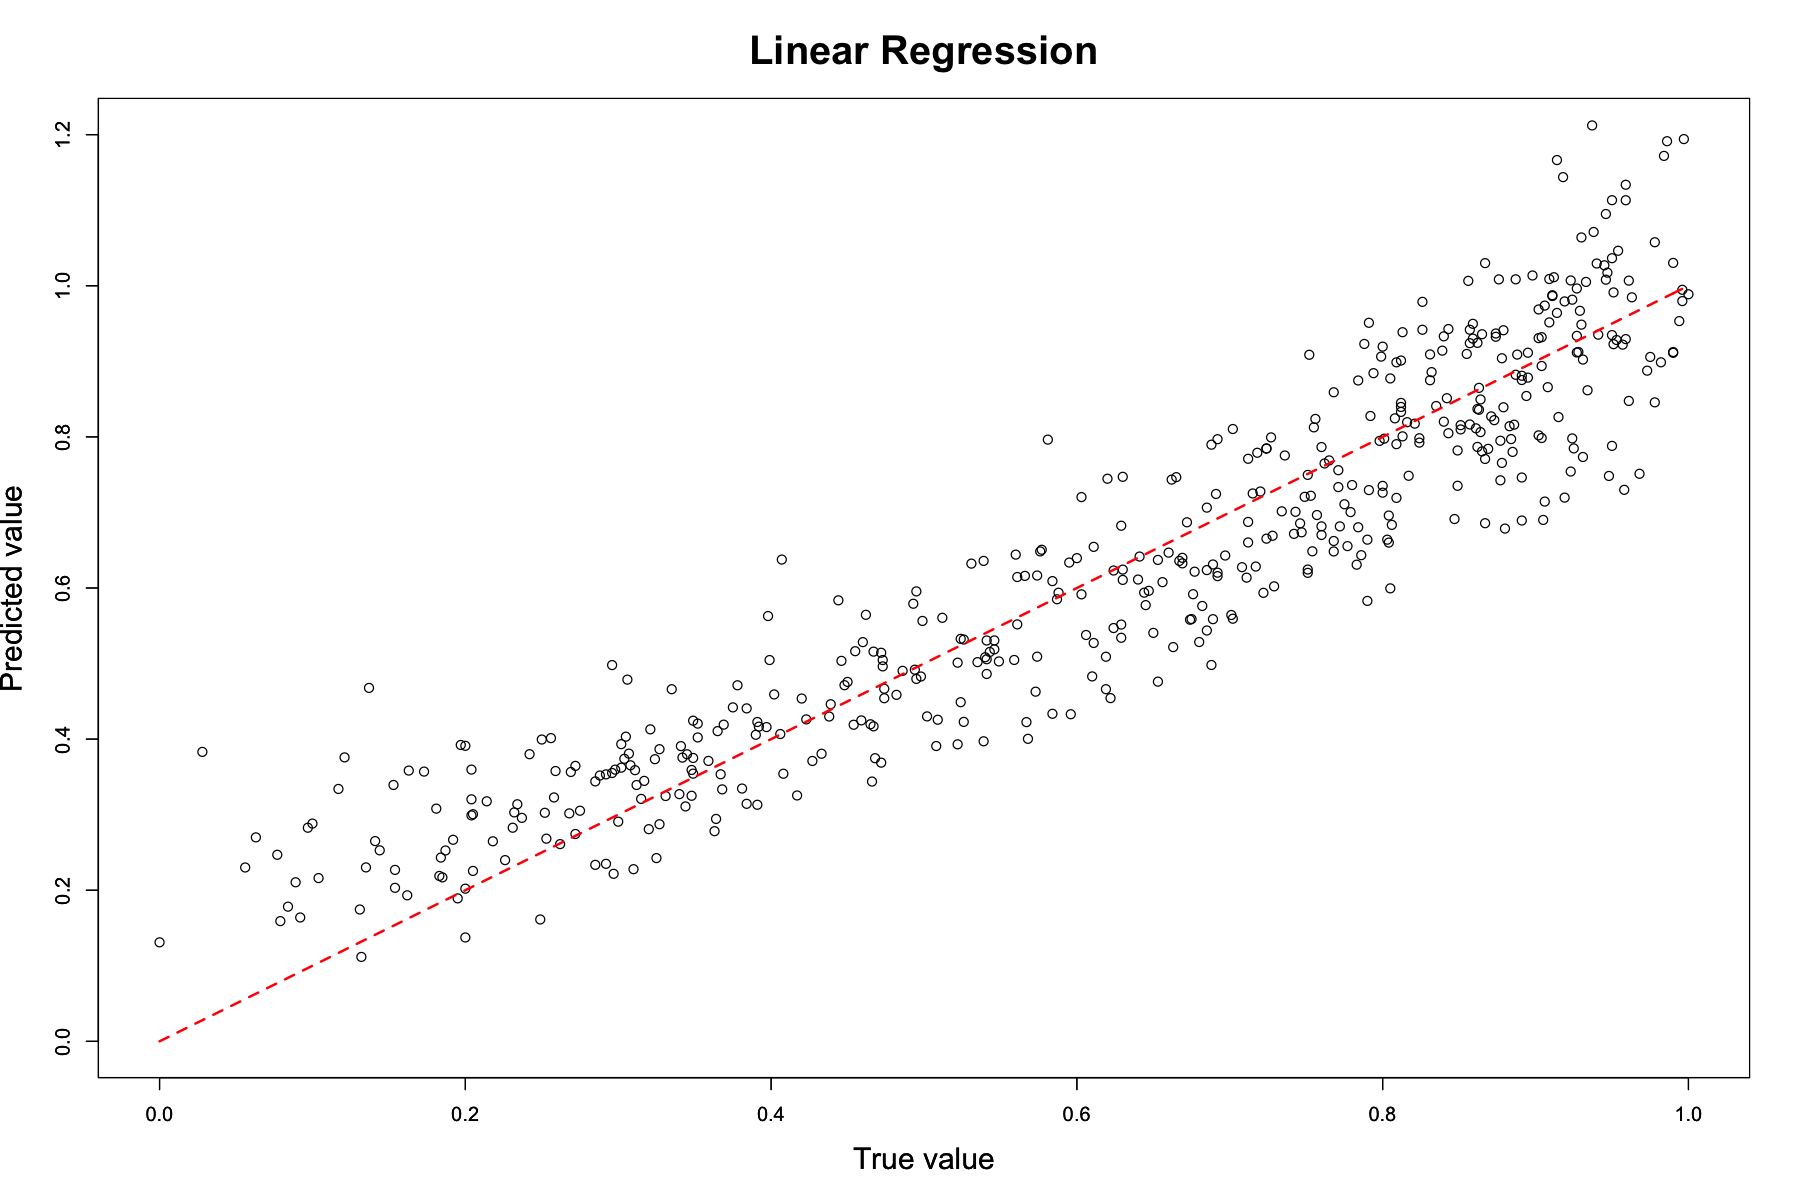
\includegraphics[width = 1.0\textwidth]{Figure/4.2.1-LR.png}
\caption{The predicted Arctic sea ice extent value vs the real Arctic sea ice extent value with Linear Regression. The red referenced dotted line represents the straight line y=x. Mean Square Error (MSE) is 0.00946.}
\label{4.2.1-LR}
\end{figure}


Using Figure \ref{4.2.1-LR}, it could be clearly found that the prediction result of Linear Regression has large error. In this case, a high $\text{R}^2$ corresponds to very poor test results. We guessed that there was an overfitting problem in the model, so we added a penalty term in the following training.



\subsection{Penalised Linear Regression (Lasso, min/1se)} %4.2.2

In order to simplify the model (reduce the number of features) while increasing the accuracy, Lasso penalization was applied on Penalized Linear Regression. Using the “glmnet” package, the weight of all features was drawn with the change of Lambda value. As the ridge-trance figure (Figure \ref{4.2.2-NEW-PLR-ridge-trance-Log-Lambda}) shows, as Lambda is worth increasing, more and more of the weights go to 0. Lasso Penalization is also based on this feature, when the Lambda increases, the feature with poor performance is gradually removed to realize the reduction of model complexity. 


\begin{figure}[htbp]
    \center
    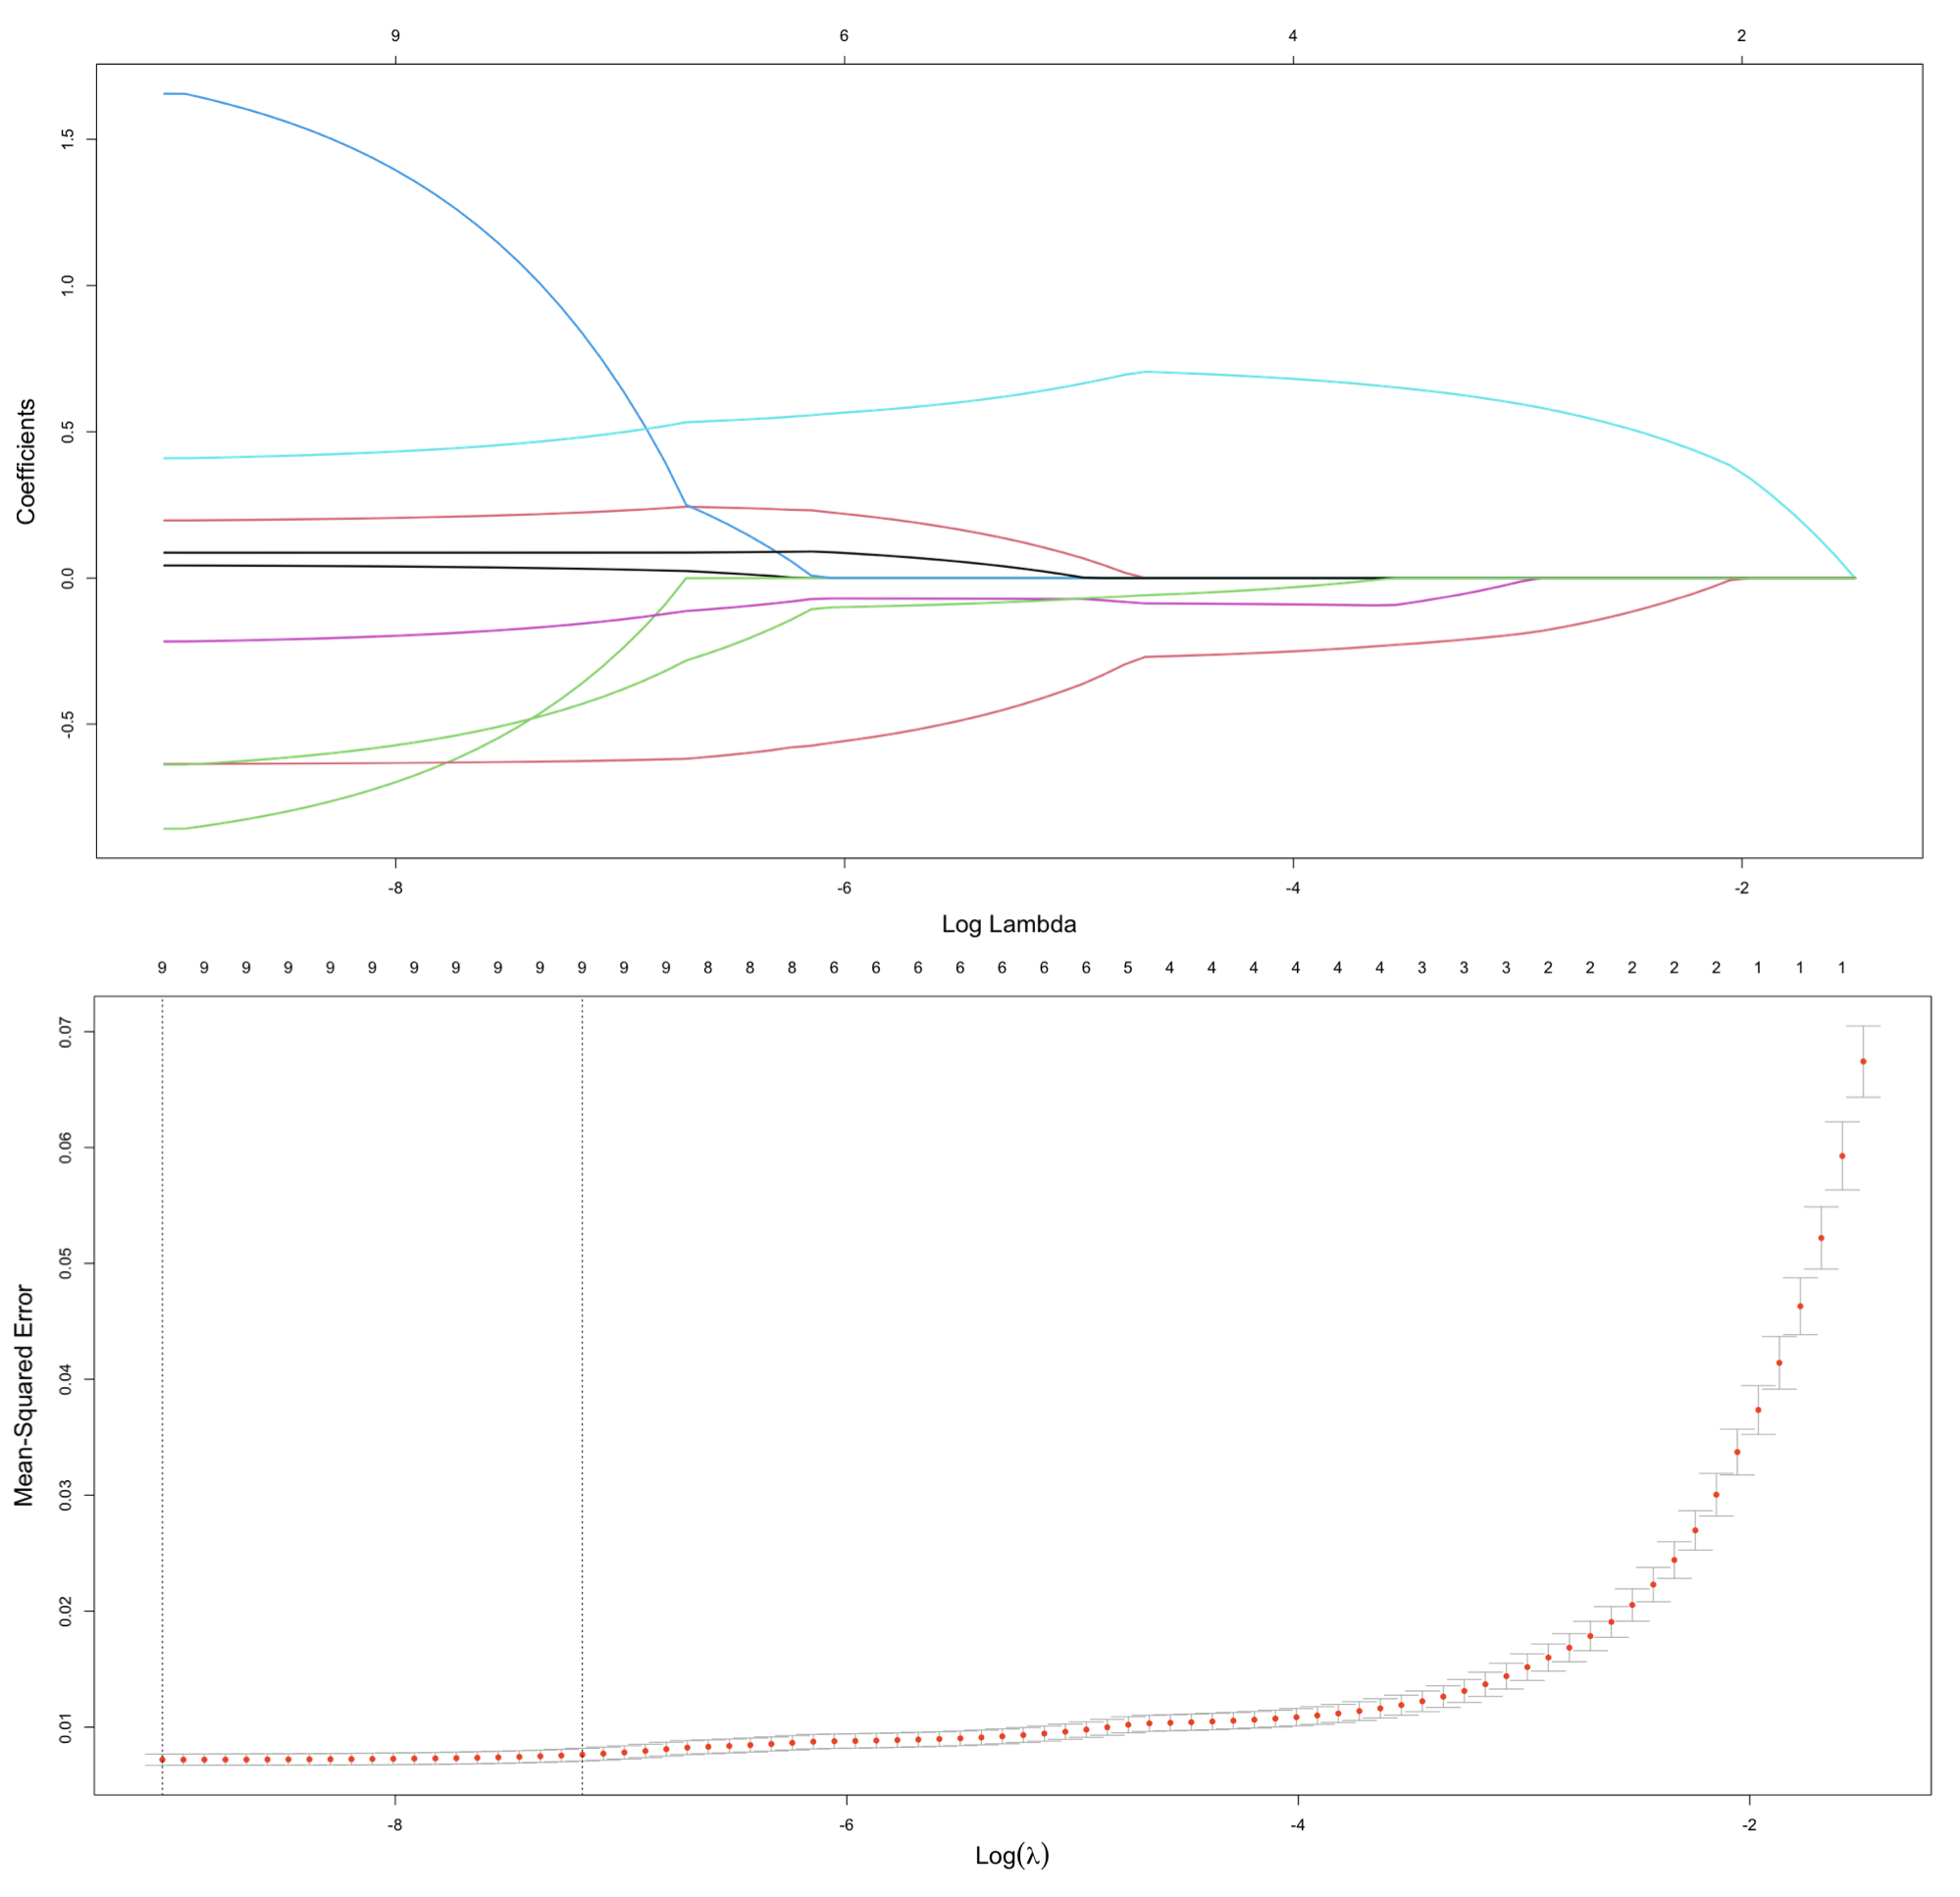
\includegraphics[scale=0.4]{Figure/4.2.2-NEW-PLR-ridge-trance-Log-Lambda.png}
    \caption{Top: Ridge trace diagram of Penalised Linear Regression; Bottom: Log Lambda vs Testing Error diagram of Penalised Linear Regression}
    \label{4.2.2-NEW-PLR-ridge-trance-Log-Lambda}
\end{figure}

%\begin{figure}[htbp]
%\centering
%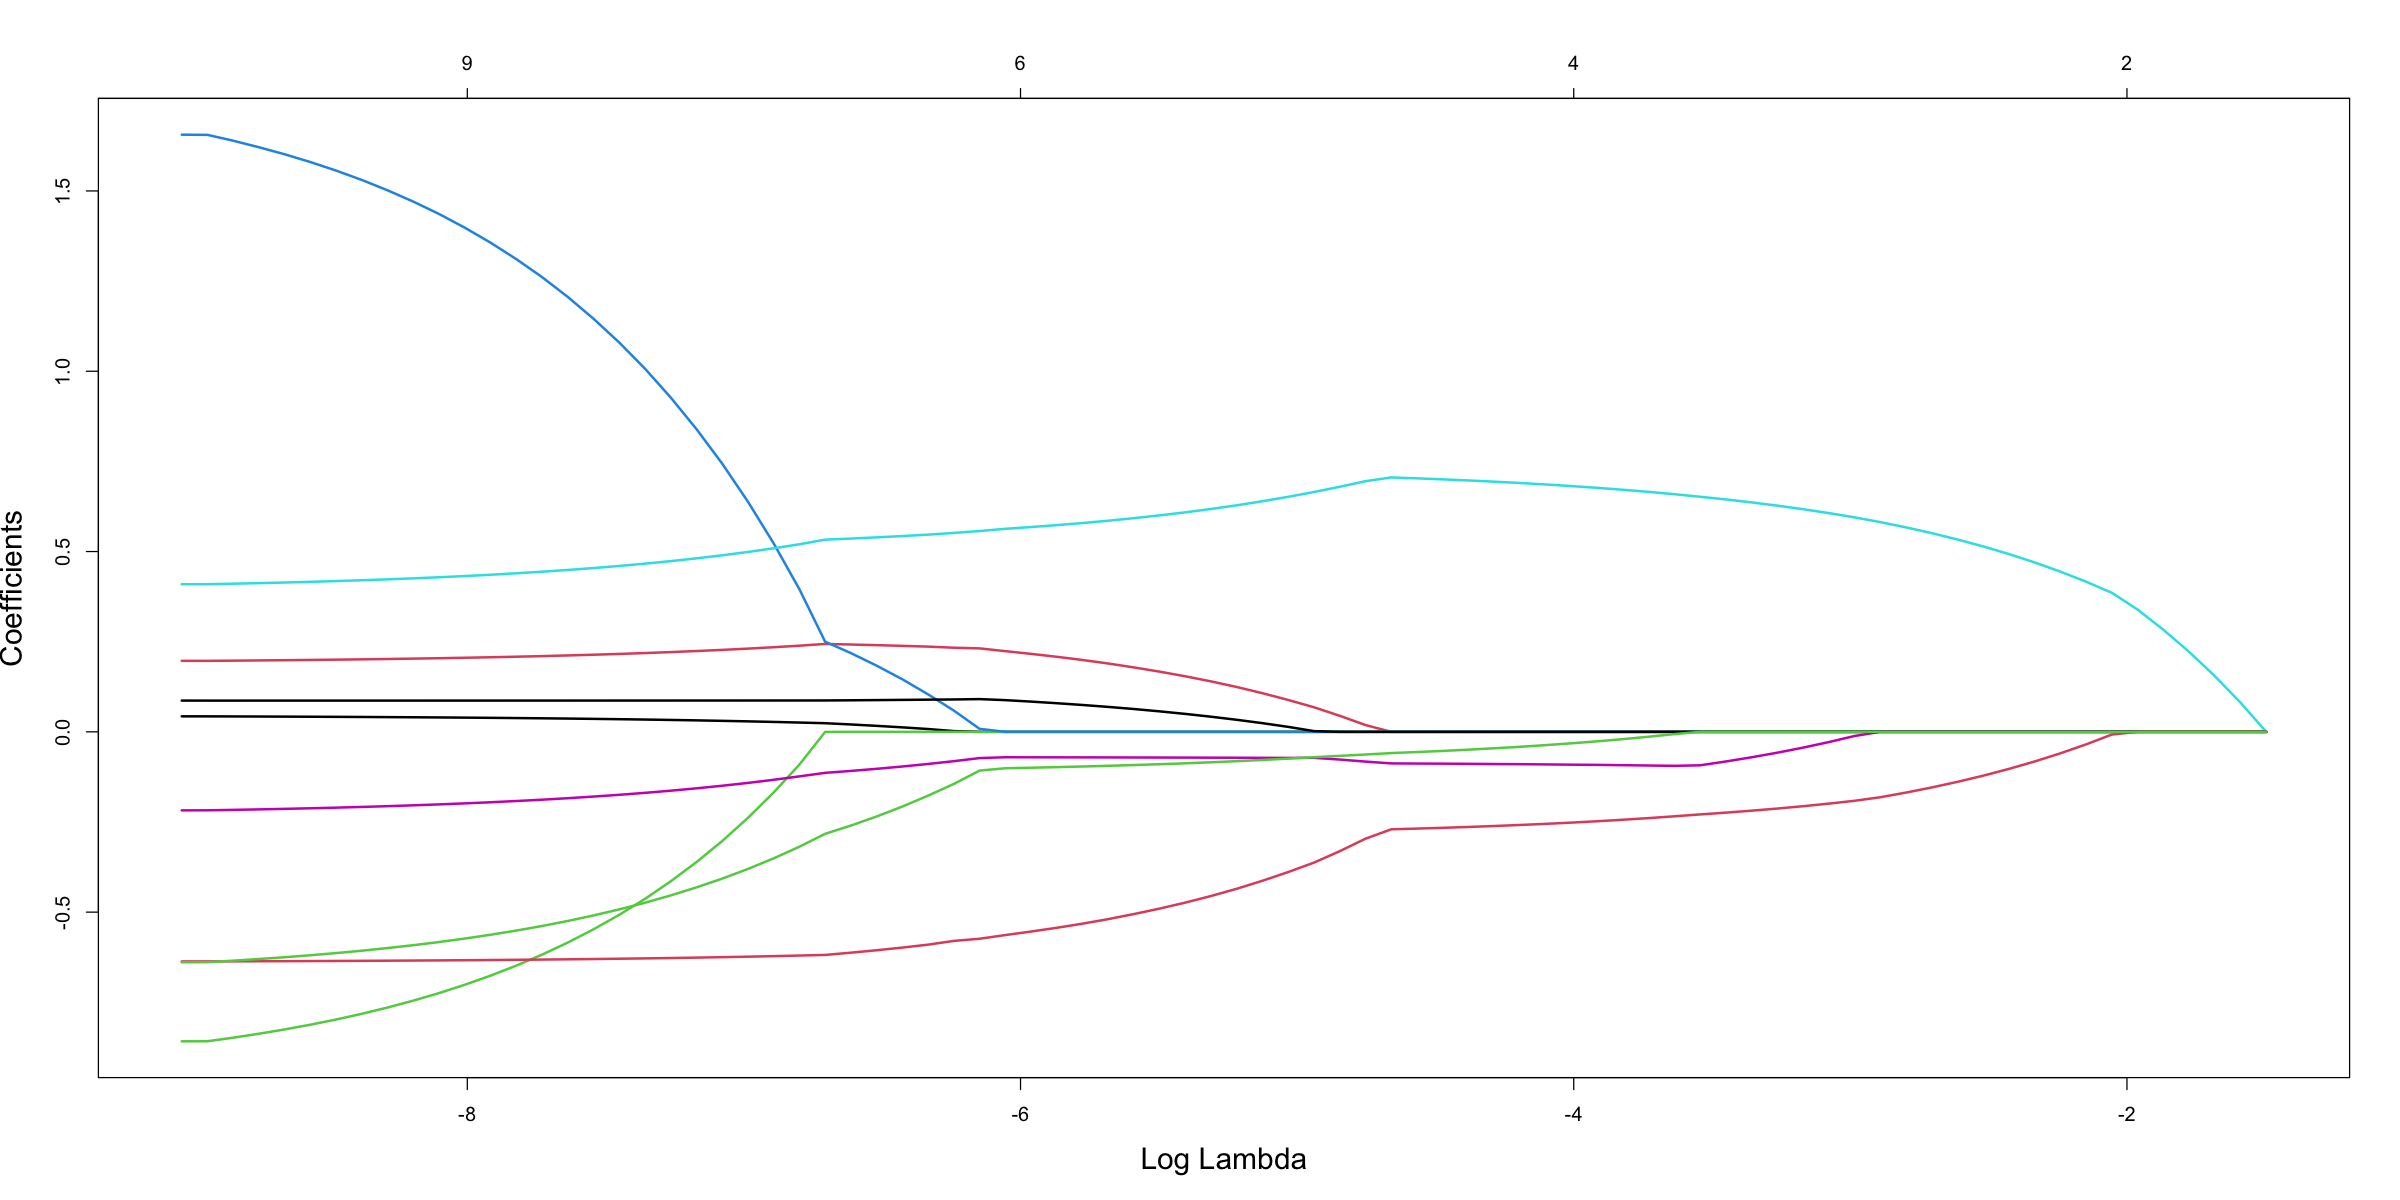
\includegraphics[width = 1.0\textwidth]{Figure/4.2.2-PLR-ridge-trance.png}
%\caption{Ridge trace diagram of Penalised Linear Regression}
%\label{4.2.2-PLR-ridge-trance}
%\end{figure}

At this point, appropriate Lambda values were needed to be selected to output weights of all features. In the selection, min and 1se option were applied respectively (Such as the x value corresponding to the two dotted lines in following Figure \ref{4.2.2-NEW-PLR-ridge-trance-Log-Lambda}).

%\begin{figure}[htbp]
%\centering
%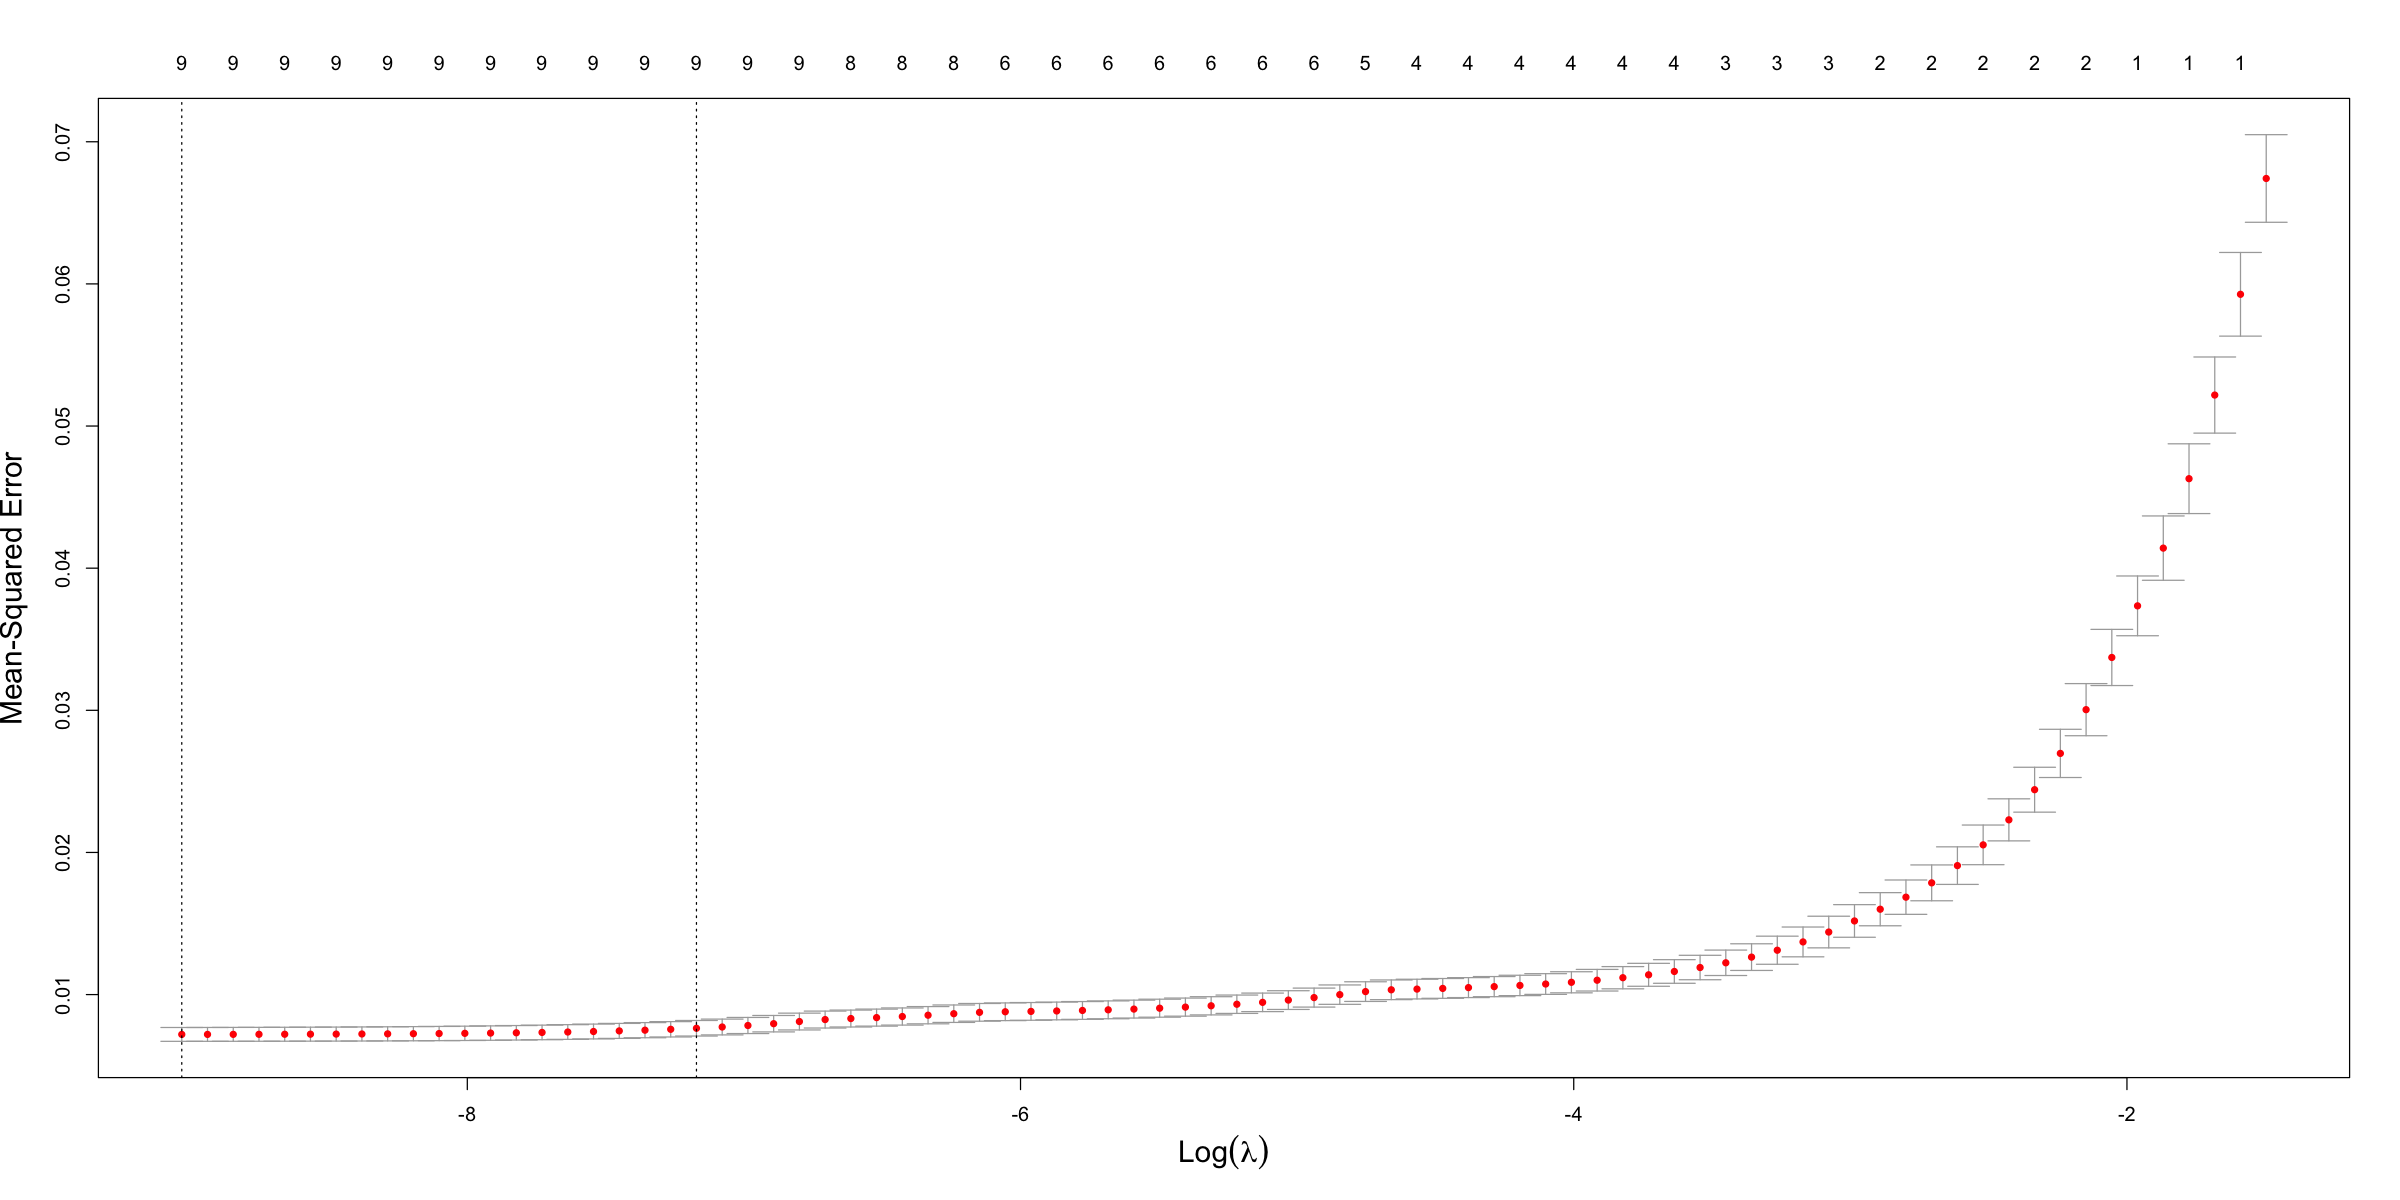
\includegraphics[width = 1.0\textwidth]{Figure/4.2.2-PLR-Log-Lambda-vs-Testing-Error.png}
%\caption{Log Lambda vs Testing Error diagram of Penalised Linear %Regression}
%\label{4.2.2-PLR-Log-Lambda-vs-Testing-Error}
%\end{figure}

Applying different option of Lambda value, two different sets of results were obtained. When Lambda option is min, the MSE value of the model is 0.00690, which is slightly less than the 0.00734 that obtained when Lambda option is 1se. The output result is shown in following Table \ref{4.2.2-PLR-para}. In this case, using 1se will not reduce the complexity of the model (reduce the number of features) but it will lose the accuracy. Therefore, in this Lasso Regression, min value is the better choice for Lambda.

\begin{table}[t]
  \centering
  \footnotesize
  \begin{tabular}{p{5.75cm} | r | r}
  \toprule
  Coefficients: & min & 1se\\ %row 1
  \hline
    & 1 & 1\\
  (Intercept) & 0.71559335 & 0.66666336\\
  Rainfall & 0.04299020 & 0.03049067\\
  Daylight & 0.19686230 & 0.22725958\\
  Population & -0.85828586 & -0.30290499\\
  CO2 & 1.65605218 & 0.74378027\\
  Ozone & 0.40941811 & 0.48953790\\
  OceanTemperature\_NorthernHemisphere & -0.21778615 & -0.14950798\\
  LandTemperature\_NorthernHemisphere & 0.08669526 & 0.08684475\\
  MinTemperature\_NorthSlopeAlaska & -0.63667606 & -0.62486026\\
  GDP\_WORLD & -0.63894945 & -0.40706240\\
  \bottomrule
  \end{tabular}
  \caption{Hyper-parameters of Penalised Linear Regression.}
  \label{4.2.2-PLR-para}
\end{table}


In terms of fitting, the performance of the two (applying min, 1se value of Lambda) are general and basically the same. Compared with the normal Linear Regression before the penalty term was applied, the performance of the test fitting is optimized but still not ideal. This is due to the lack of flexibility in the model.


\begin{figure}[htbp]
\centering
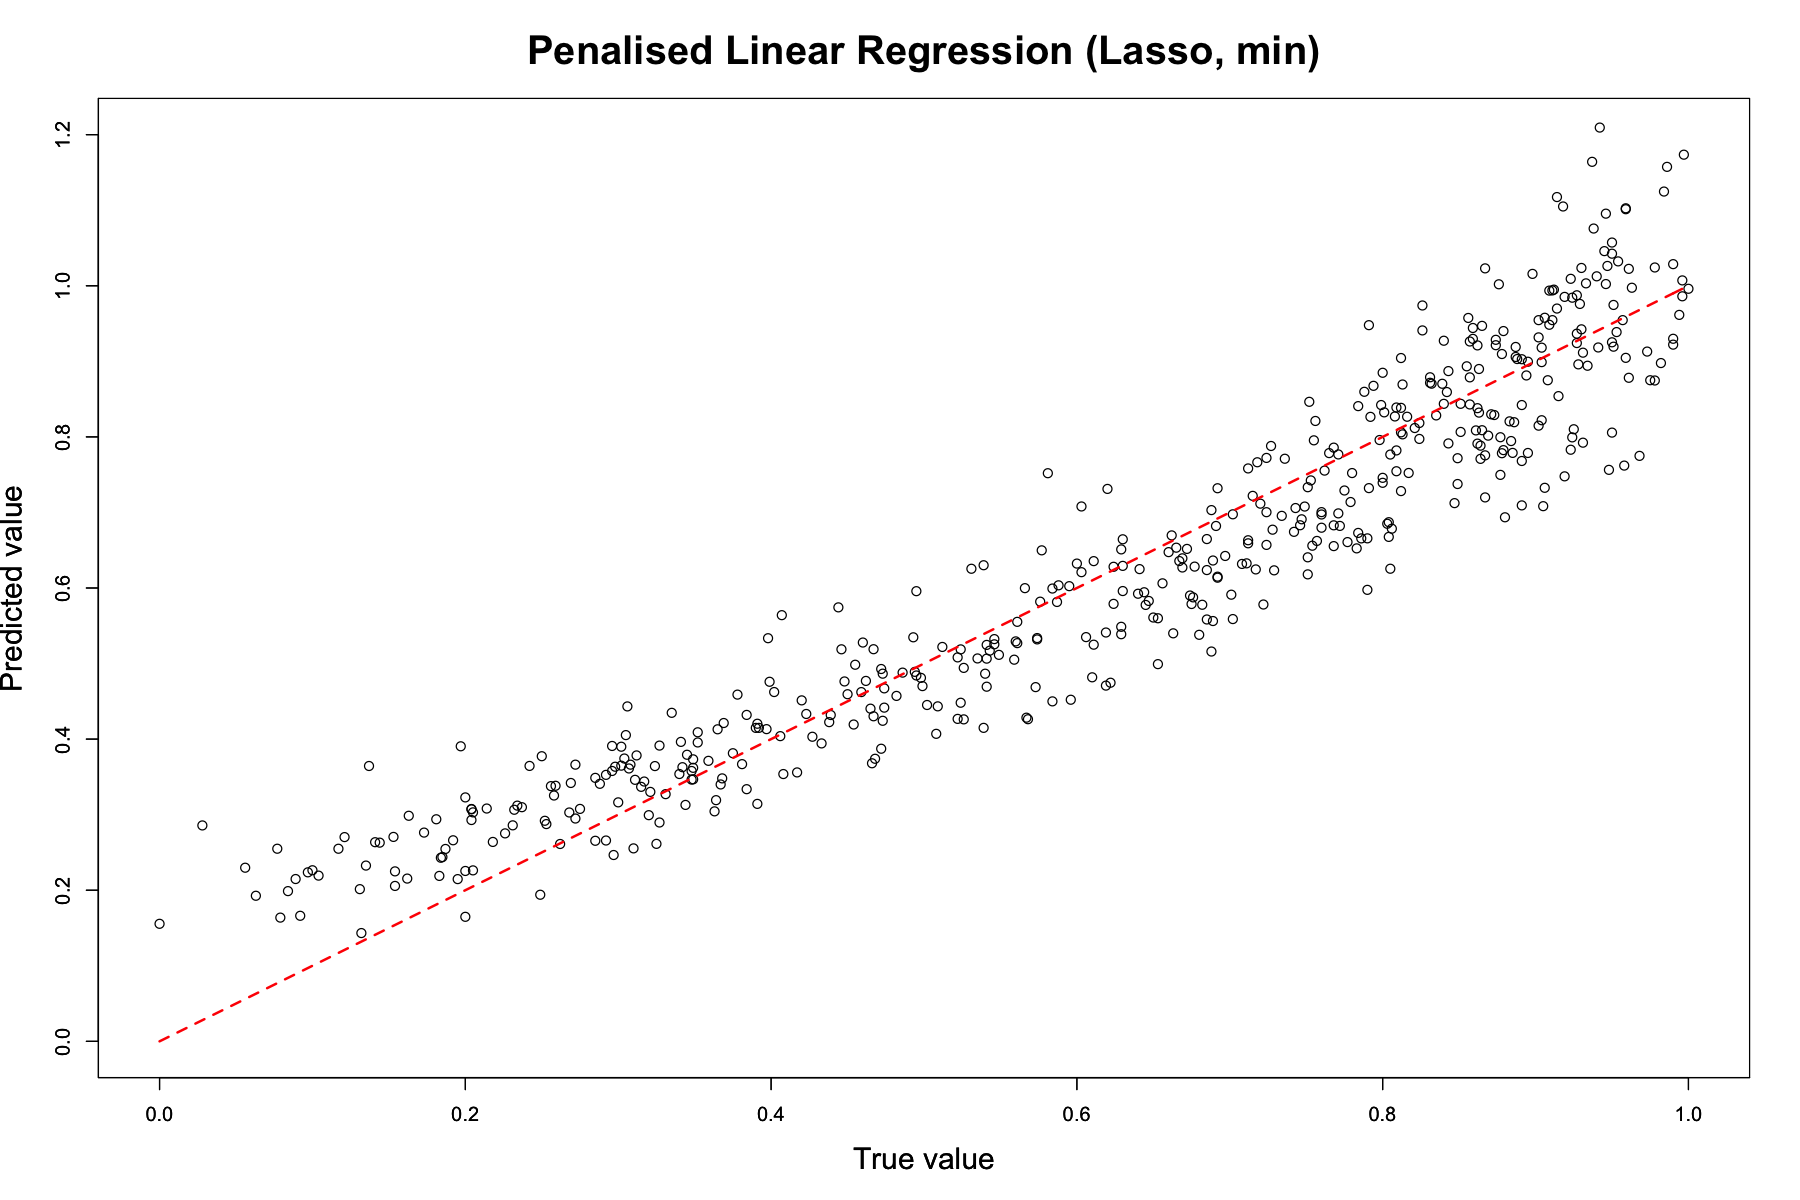
\includegraphics[width = 1.0\textwidth]{Figure/4.2.2-PLR-min.png}
\caption{The predicted Arctic sea ice extent value vs the real Arctic sea ice extent value with Penalised Linear Regression (Lasso, min). The red referenced dotted line represents the straight line y=x. Mean Square Error (MSE) is 0.00690.}
\label{4.2.2-PLR-min}
\end{figure}


\begin{figure}[htbp]
\centering
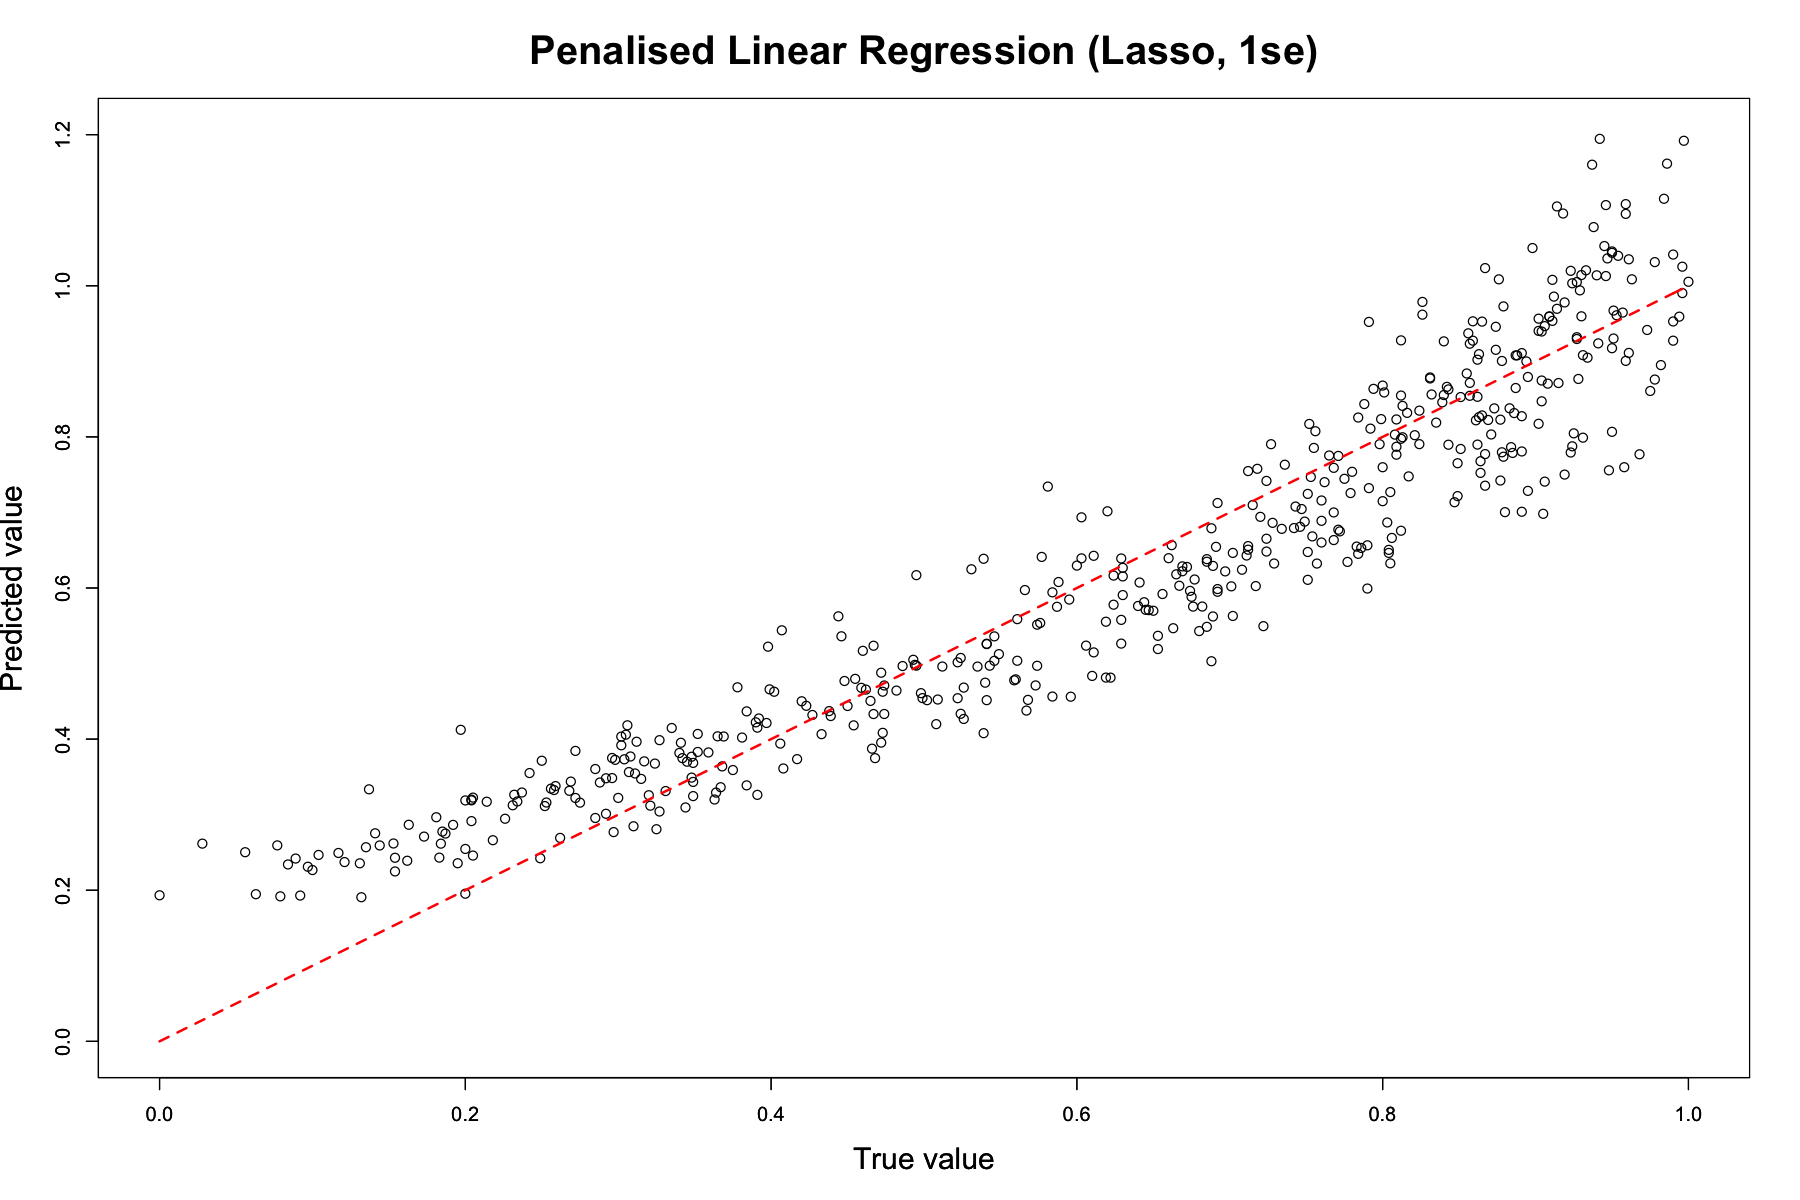
\includegraphics[width = 1.0\textwidth]{Figure/4.2.2-PLR-1se.png}
\caption{The predicted Arctic sea ice extent value vs the real Arctic sea ice extent value with Penalised Linear Regression (Lasso, 1se). The red referenced dotted line represents the straight line y=x. Mean Square Error (MSE) is 0.00732.}
\label{4.2.2-PLR-1se}
\end{figure}



\subsection{Penalised Polynomial Regression (Lasso, min/1se)} %4.2.3
To increase the flexibility of the model, polynomial regression was applied. Based on the correlation matrix, the four features with the best correlation were selected for this model. The order of one to four of each feature was added to the training. Similarly, polynomial regression suffered from overfitting, so the Lasso penalty term was still used in this model.

Again, ridge-trance graph was generated.

Similarly, applying log Lambda vs testing error **GRAPH**, the Lambda value can be chosen.

According to the following **RESULTS (the table)**, it can be seen that all the features (16) are kept in this model applying min Lambda value while only 10 features are kept applying 1se. In this case, unlike the previous Penalized Linear Regression, applying 1se value of Lambda achieve cancelling nearly half of the features, which is able to greatly simplifies the model. Comparing the MSE of both options, MSE equals to 0.00448 when min value is applied. In comparison, the MSE only increases to 0.00483 applying 1se. At the cost of small precision loss, the model can be greatly simplified, which is exactly the purpose of the 1se option of Lambda.

By comparing the fitting **DIAGRAM** of two results, it can be found that the results are similar, which further proves that the influence of 1se value on the accuracy of the model is almost negligible. At the same time, compared with linear regression, the fitting results were significantly better, which was due to the fact that polynomial regression brought more flexibility to the model.



\begin{figure}[htbp]
    \center
    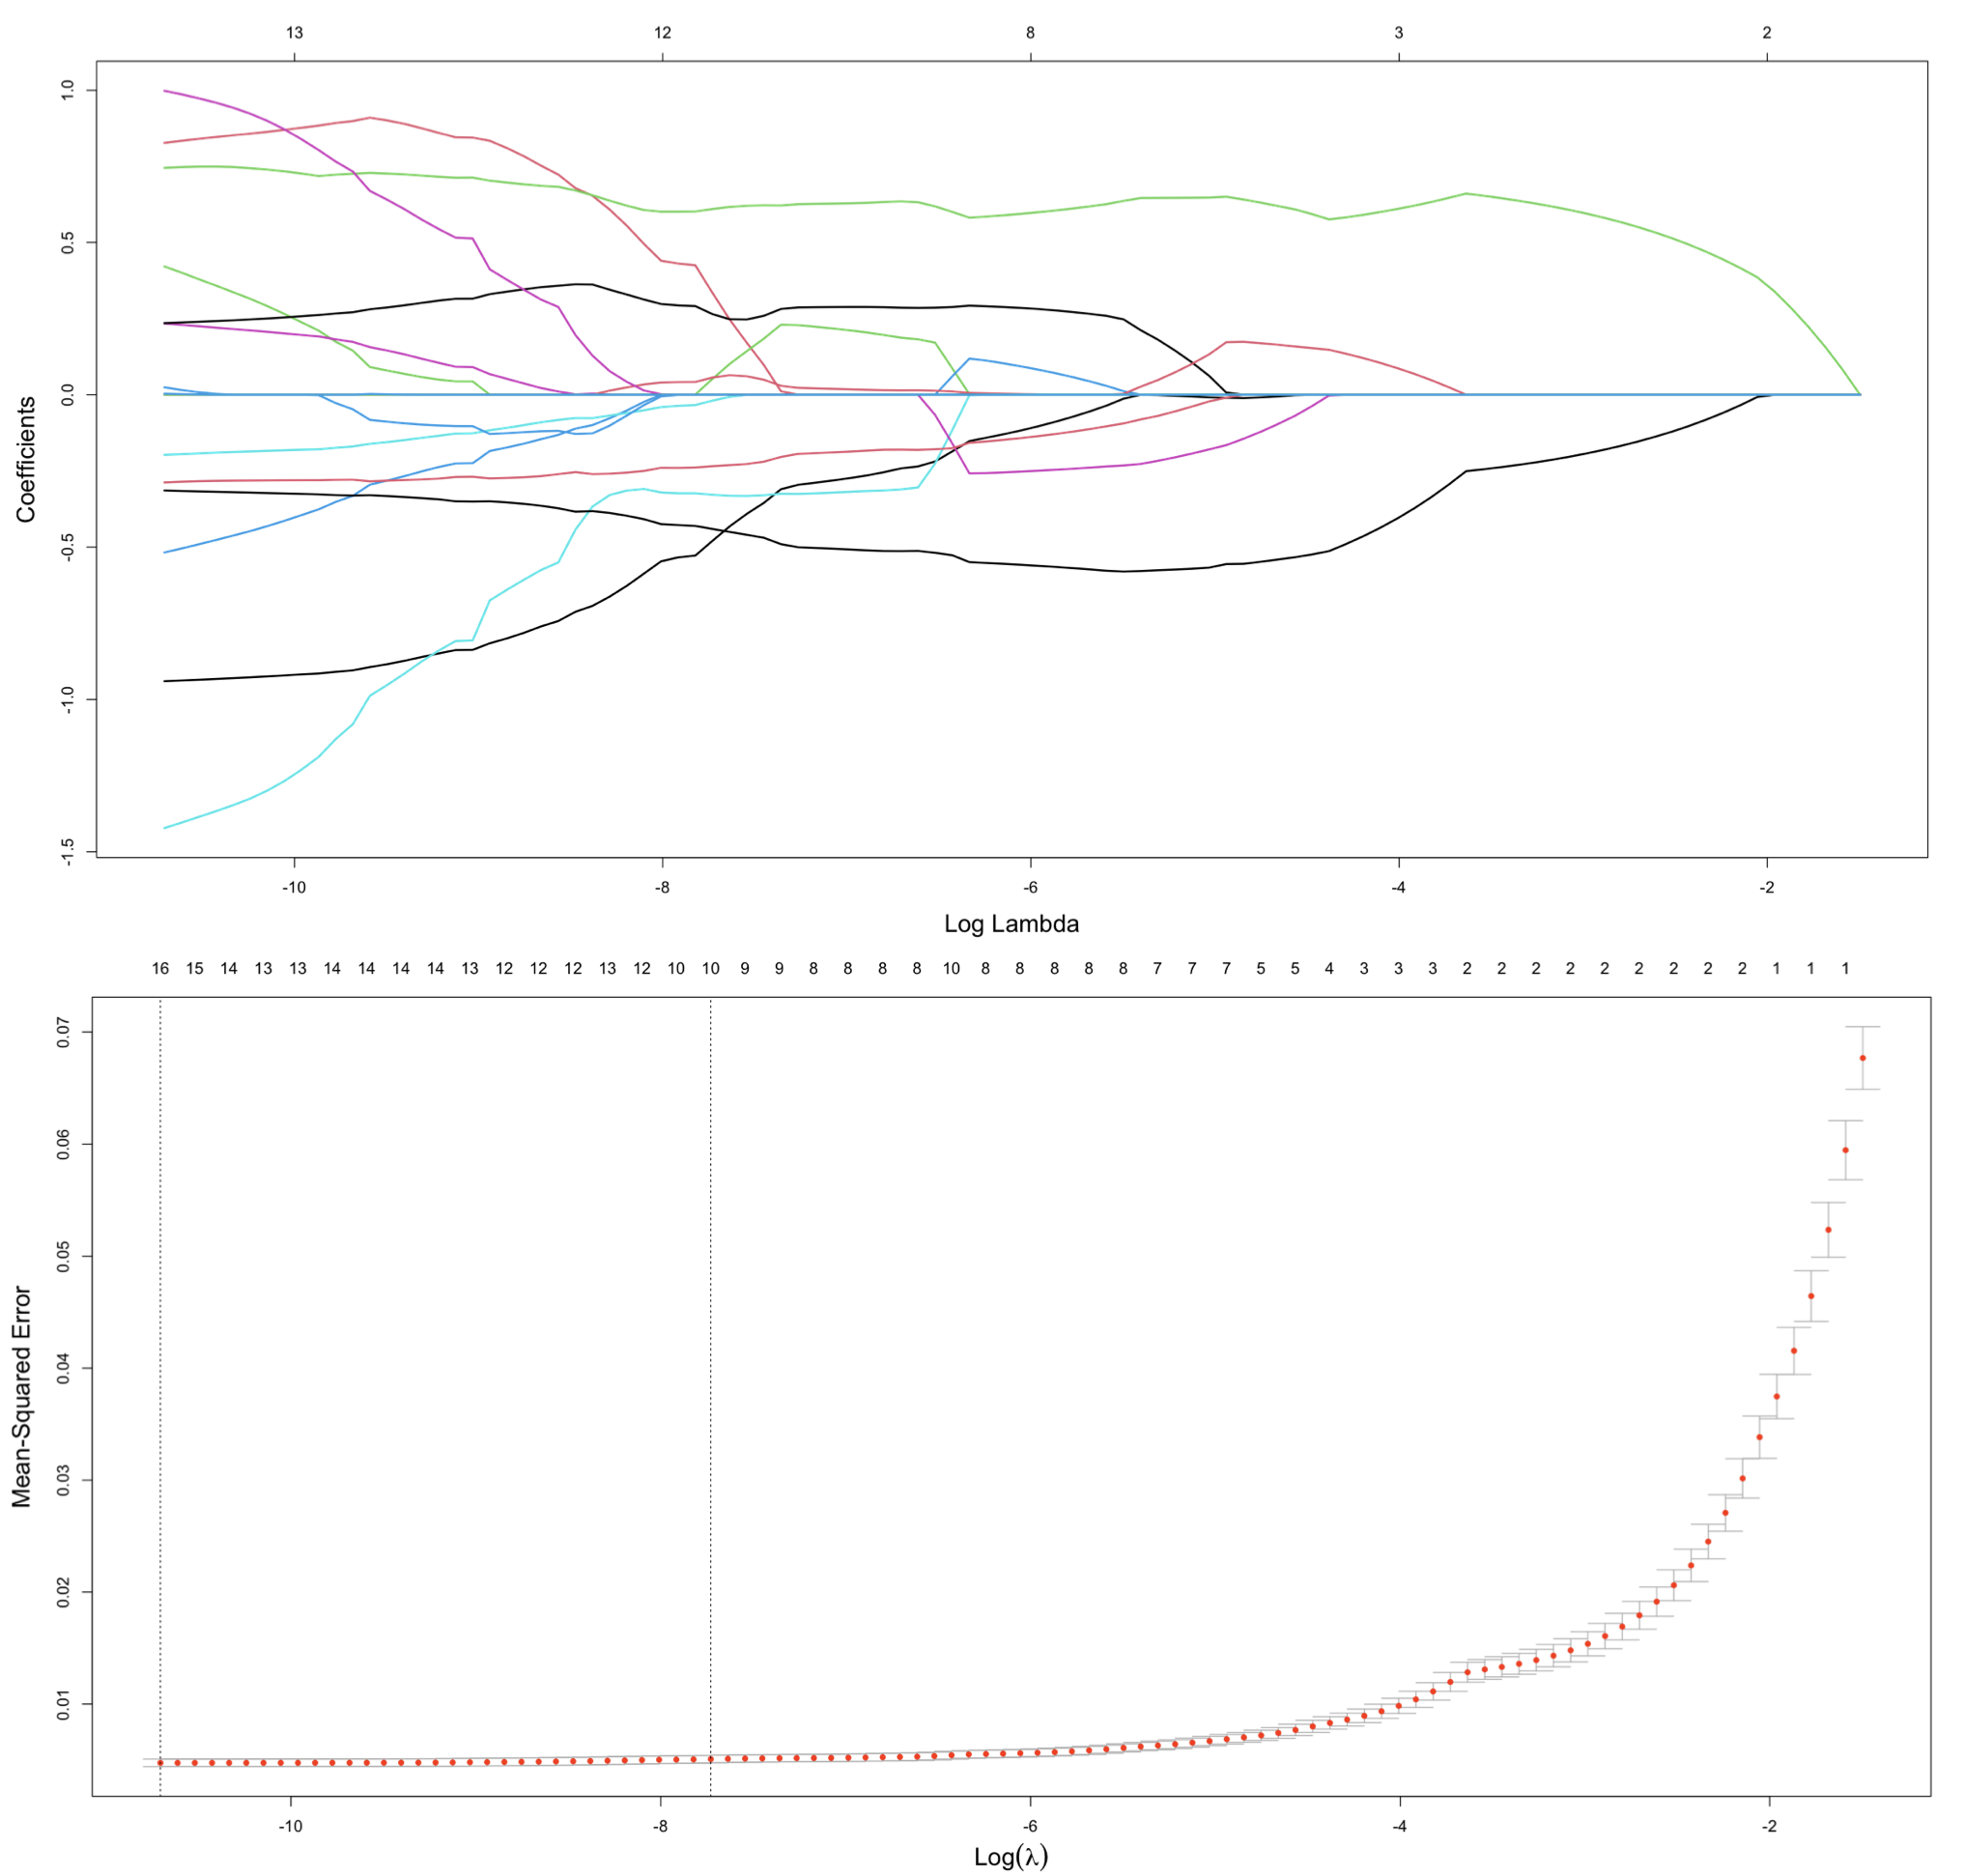
\includegraphics[scale=0.4]{Figure/4.2.3-NEW-PPR-ridge-trance-Log-Lambda.png}
    \caption{Top: Ridge trace diagram of Penalised Polynomial Regression; Bottom: Log Lambda vs Testing Error diagram of Penalised Polynomial Regression}
    \label{4.2.3-NEW-PPR-ridge-trance-Log-Lambda}
\end{figure}


\begin{figure}[htbp]
\centering
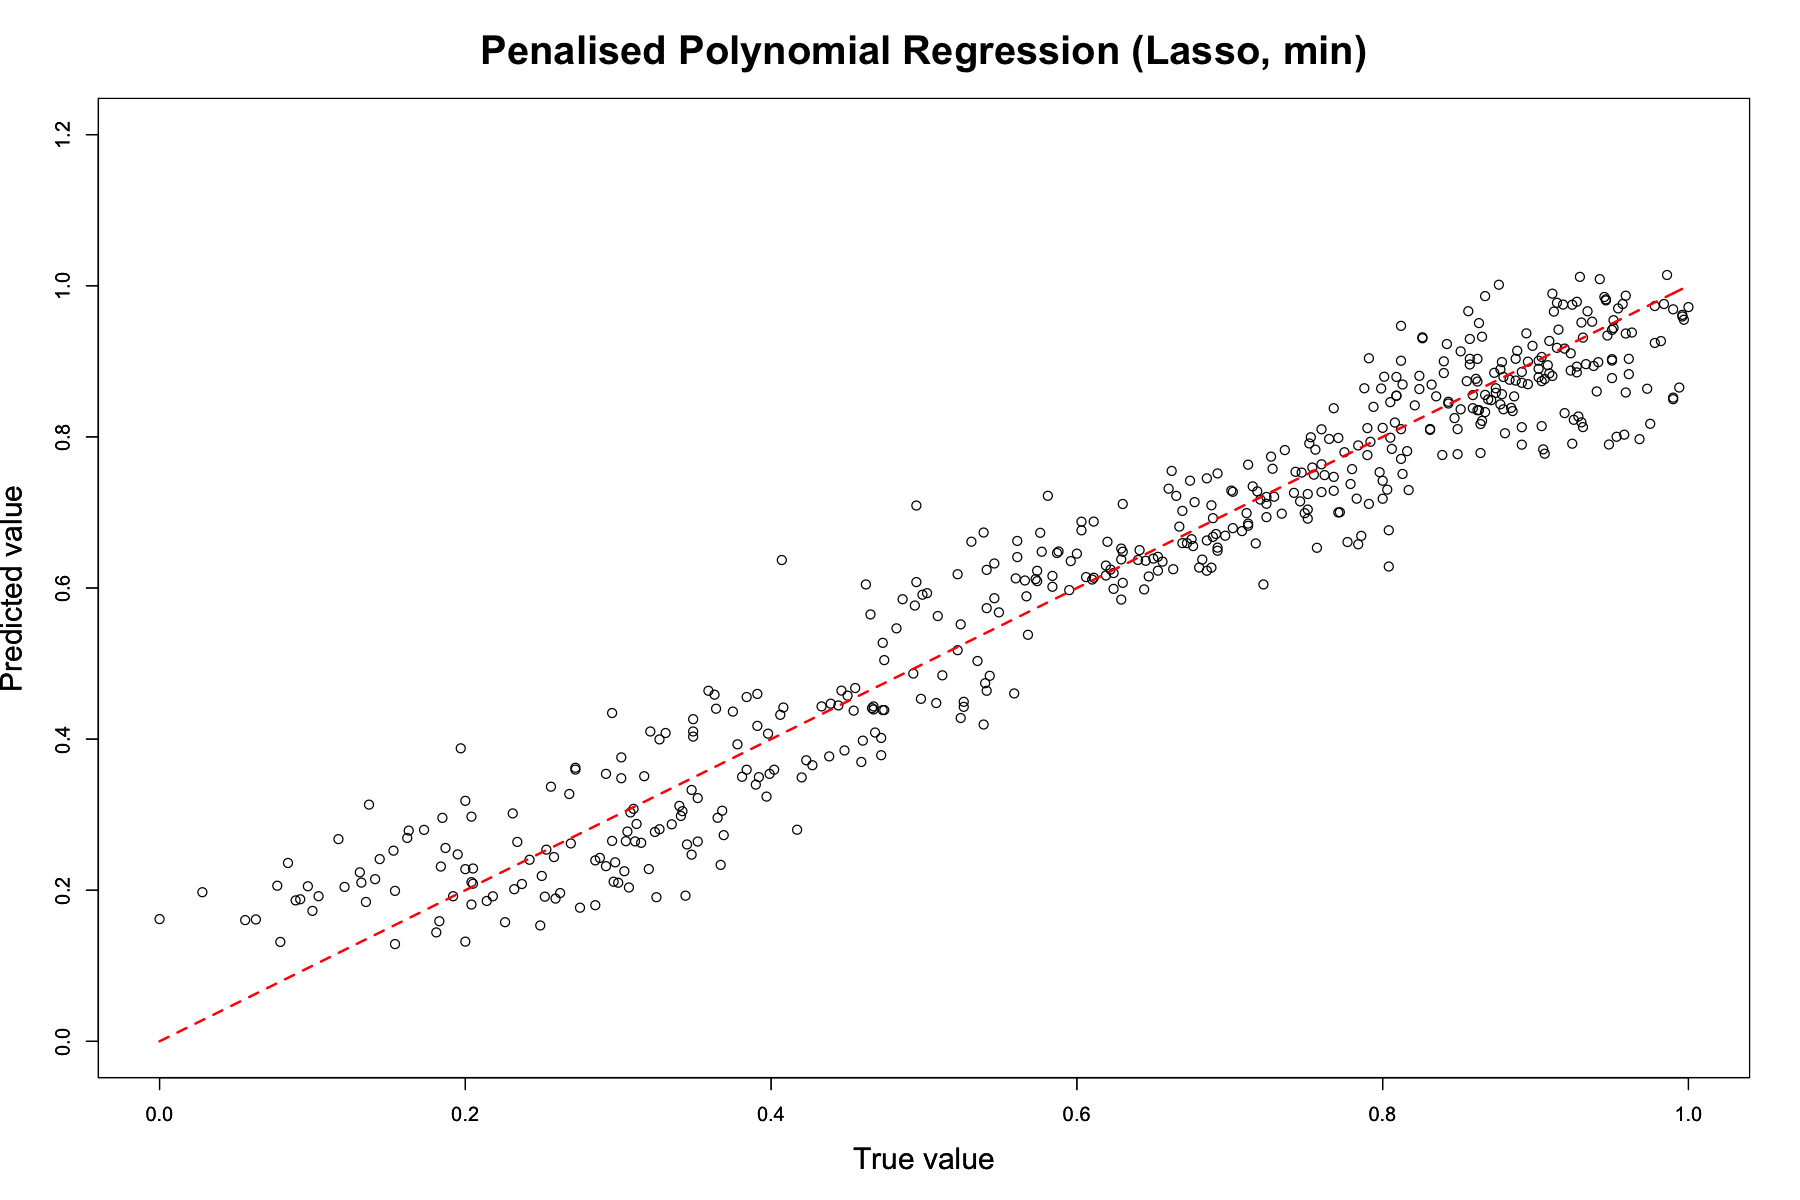
\includegraphics[width = 1.0\textwidth]{Figure/4.2.3-PPR-min.png}
\caption{The predicted Arctic sea ice extent value vs the real Arctic sea ice extent value with Penalised Polynomial Regression (Lasso, min). The red referenced dotted line represents the straight line y=x. Mean Square Error (MSE) is 0.00448.}
\label{4.2.3-PPR-min}
\end{figure}

\begin{figure}[htbp]
\centering
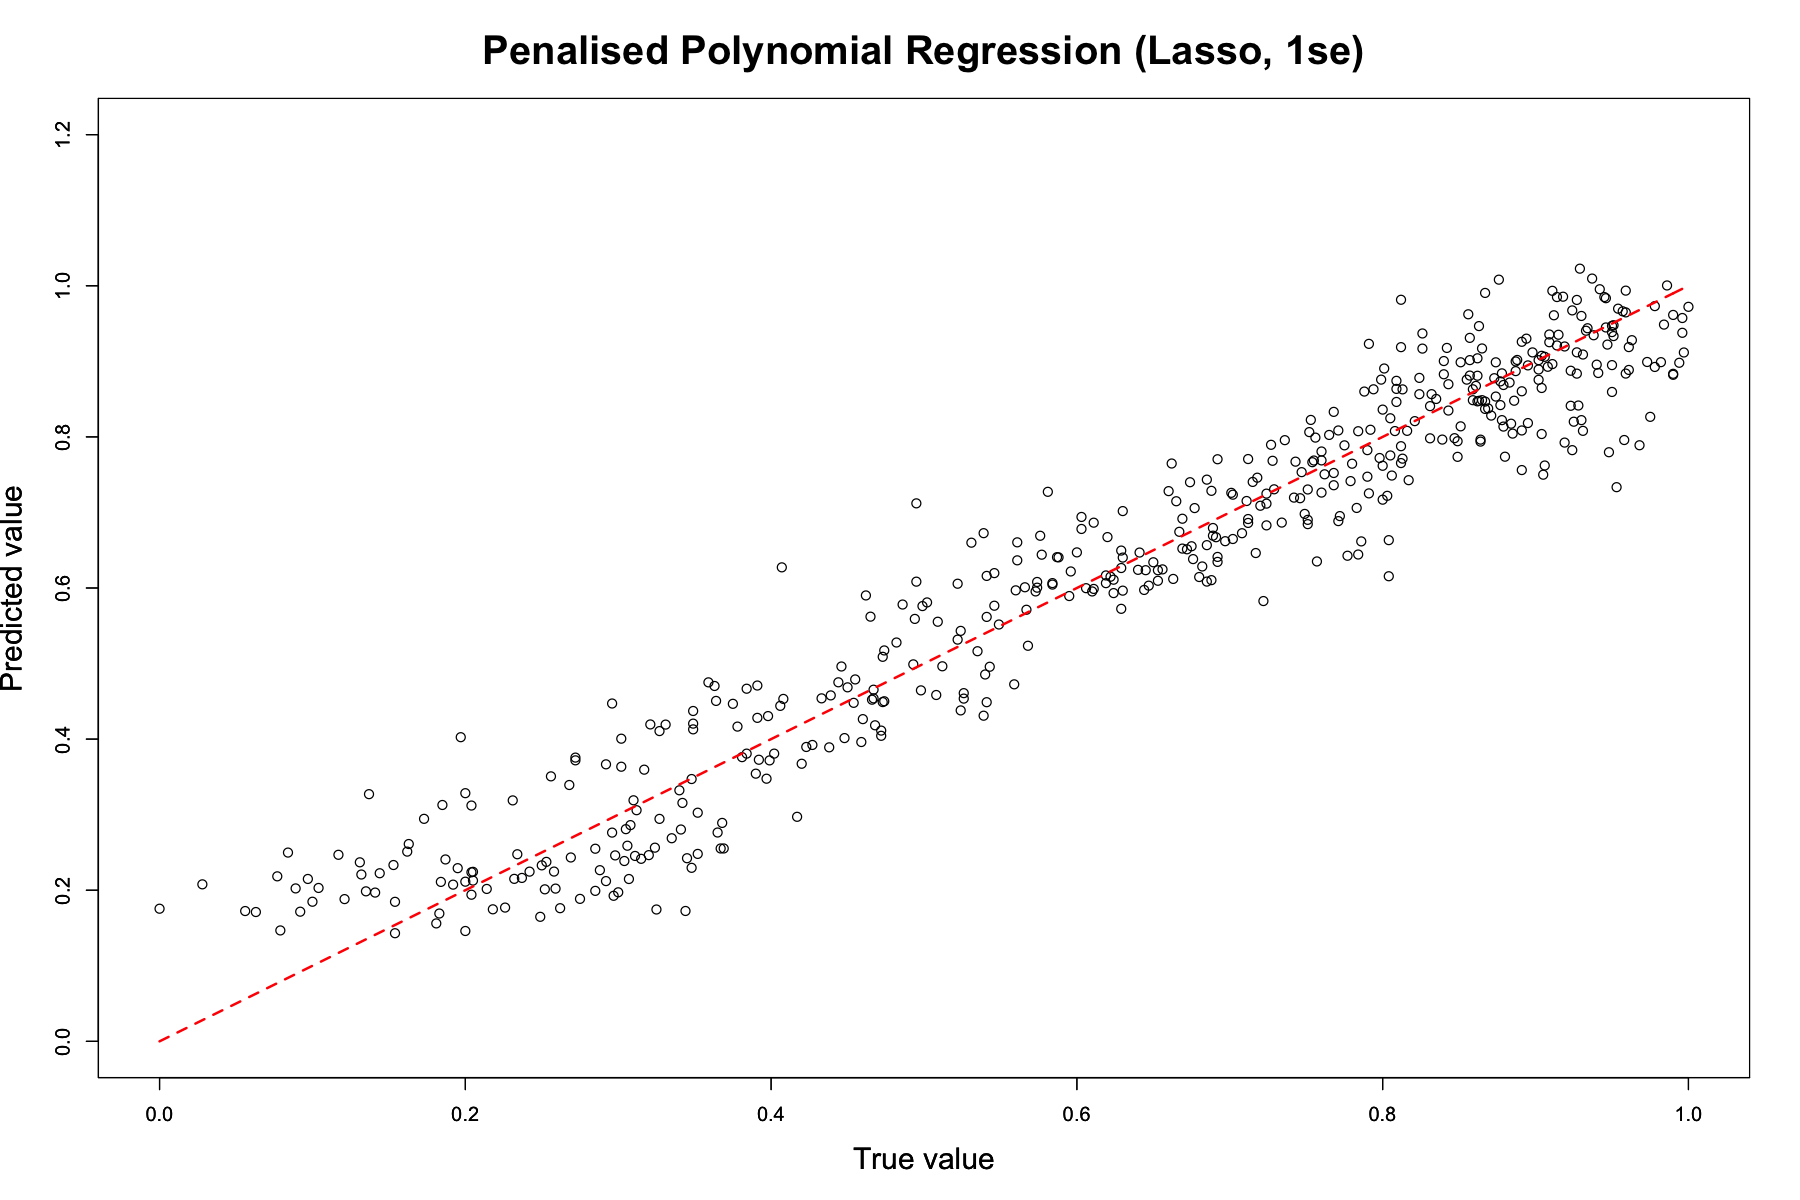
\includegraphics[width = 1.0\textwidth]{Figure/4.2.3-PPR-1se.png}
\caption{The predicted Arctic sea ice extent value vs the real Arctic sea ice extent value with Penalised Polynomial Regression (Lasso, 1se). The red referenced dotted line represents the straight line y=x. Mean Square Error (MSE) is 0.00484.}
\label{4.2.3-PPR-1se}
\end{figure}



\subsection{Random Forest} %4.2.4

To use Random Forest, three parameters need to be determined, namely, the number of total features, the number of trees, and mtry (number of features that randomly applied in each tree). Firstly, 9 out of 11 features are applied in this algorithm based on correlation matrix. Then, the “tree number vs out-of-bag error” graph (Figure \ref{4.2.6-RF-200TreesStable}) was plotted. It can be seen that, based on different mtry values, when the tree number approaches 200, the out-of-bag error tends to be stable. Therefore, 200 is chosen as the tree number of this model.

\begin{figure}[htbp]
\centering
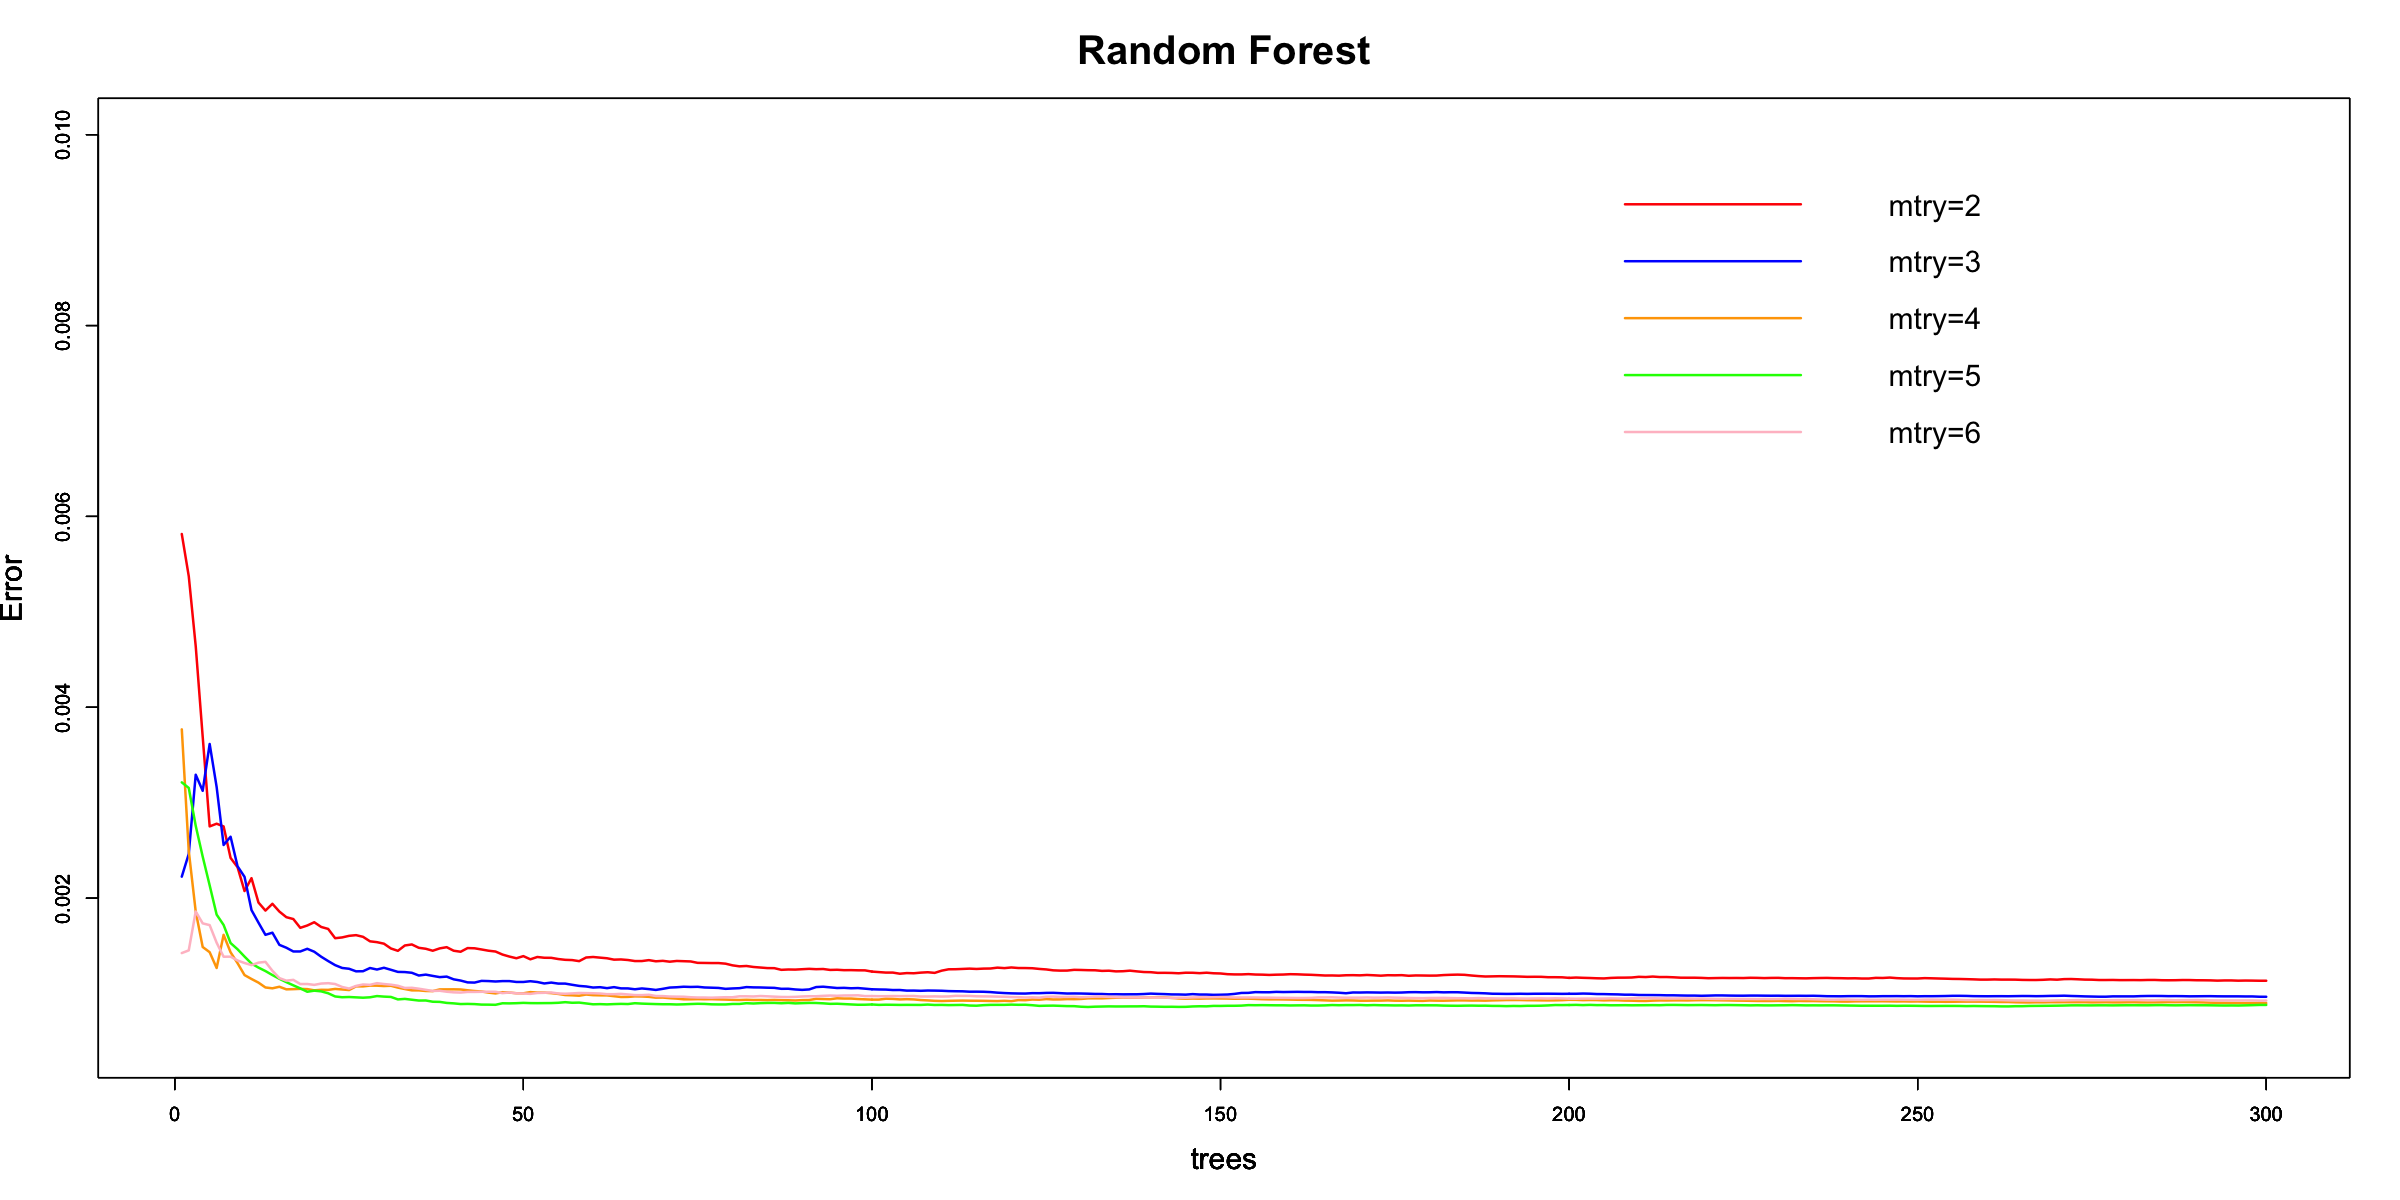
\includegraphics[width = 1.0\textwidth]{Figure/4.2.4-RF-200TreesStable.png}
\caption{Check the error stability of random forest with different number of trees.}
\label{4.2.6-RF-200TreesStable}
\end{figure}

Moreover, the choice of the mtry value is also important. Based on the already selected tree number 200. By using different mtry (from 2-6) values training models, different out-of-bag errors will be obtained. Through comparison, 5 is finally selected as mtry value, which corresponds with minimum out-of-bag error.

\begin{figure}[htbp]
\centering
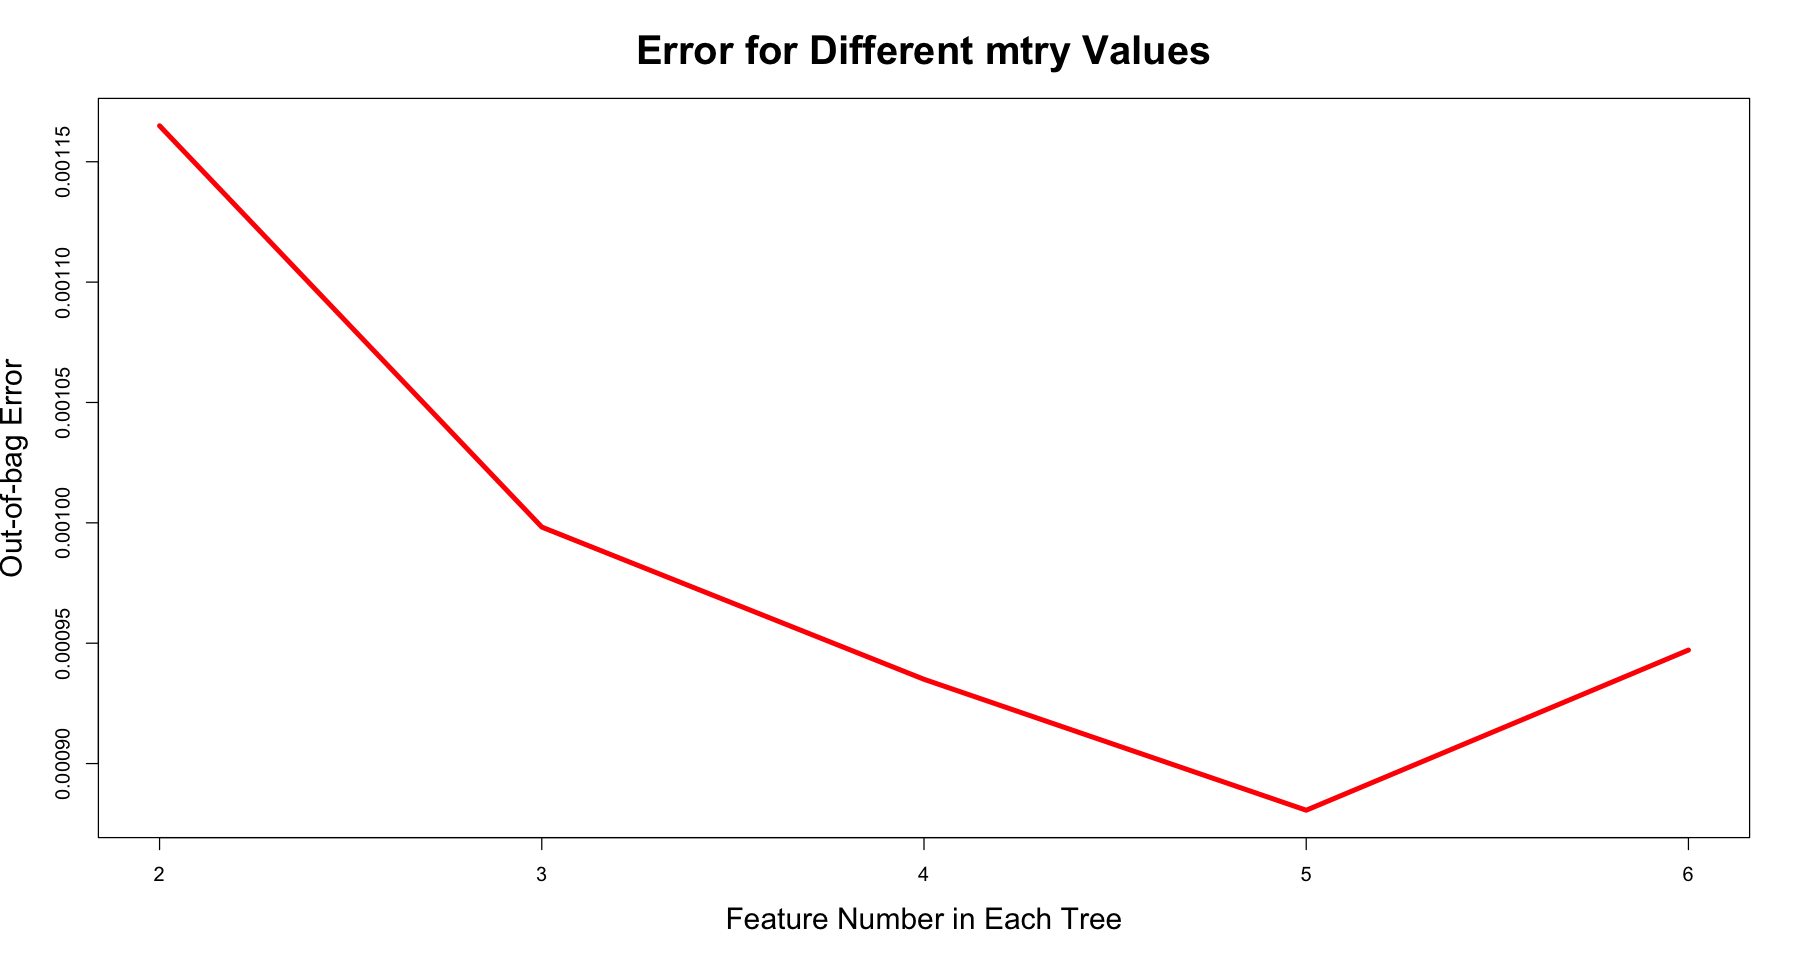
\includegraphics[width = 1.0\textwidth]{Figure/4.2.4-RF-5Features.png}
\caption{Check the out-of-bag error of random forest with different number of features in each tree when three number is 200.}
\label{4.2.4-RF-5Features}
\end{figure}

After Parameter selection, Random Forest model can be trained and tested. The MSE output is 0.00105, which is much lower than the previous models. Observing the fitting diagram (Figure \ref{4.2.4-RF}), it can be found that the dots are distributed in a narrow area fitting the straight line x=y, which indicated the performance of Random Forest is satisfying.

\begin{figure}[htbp]
\centering
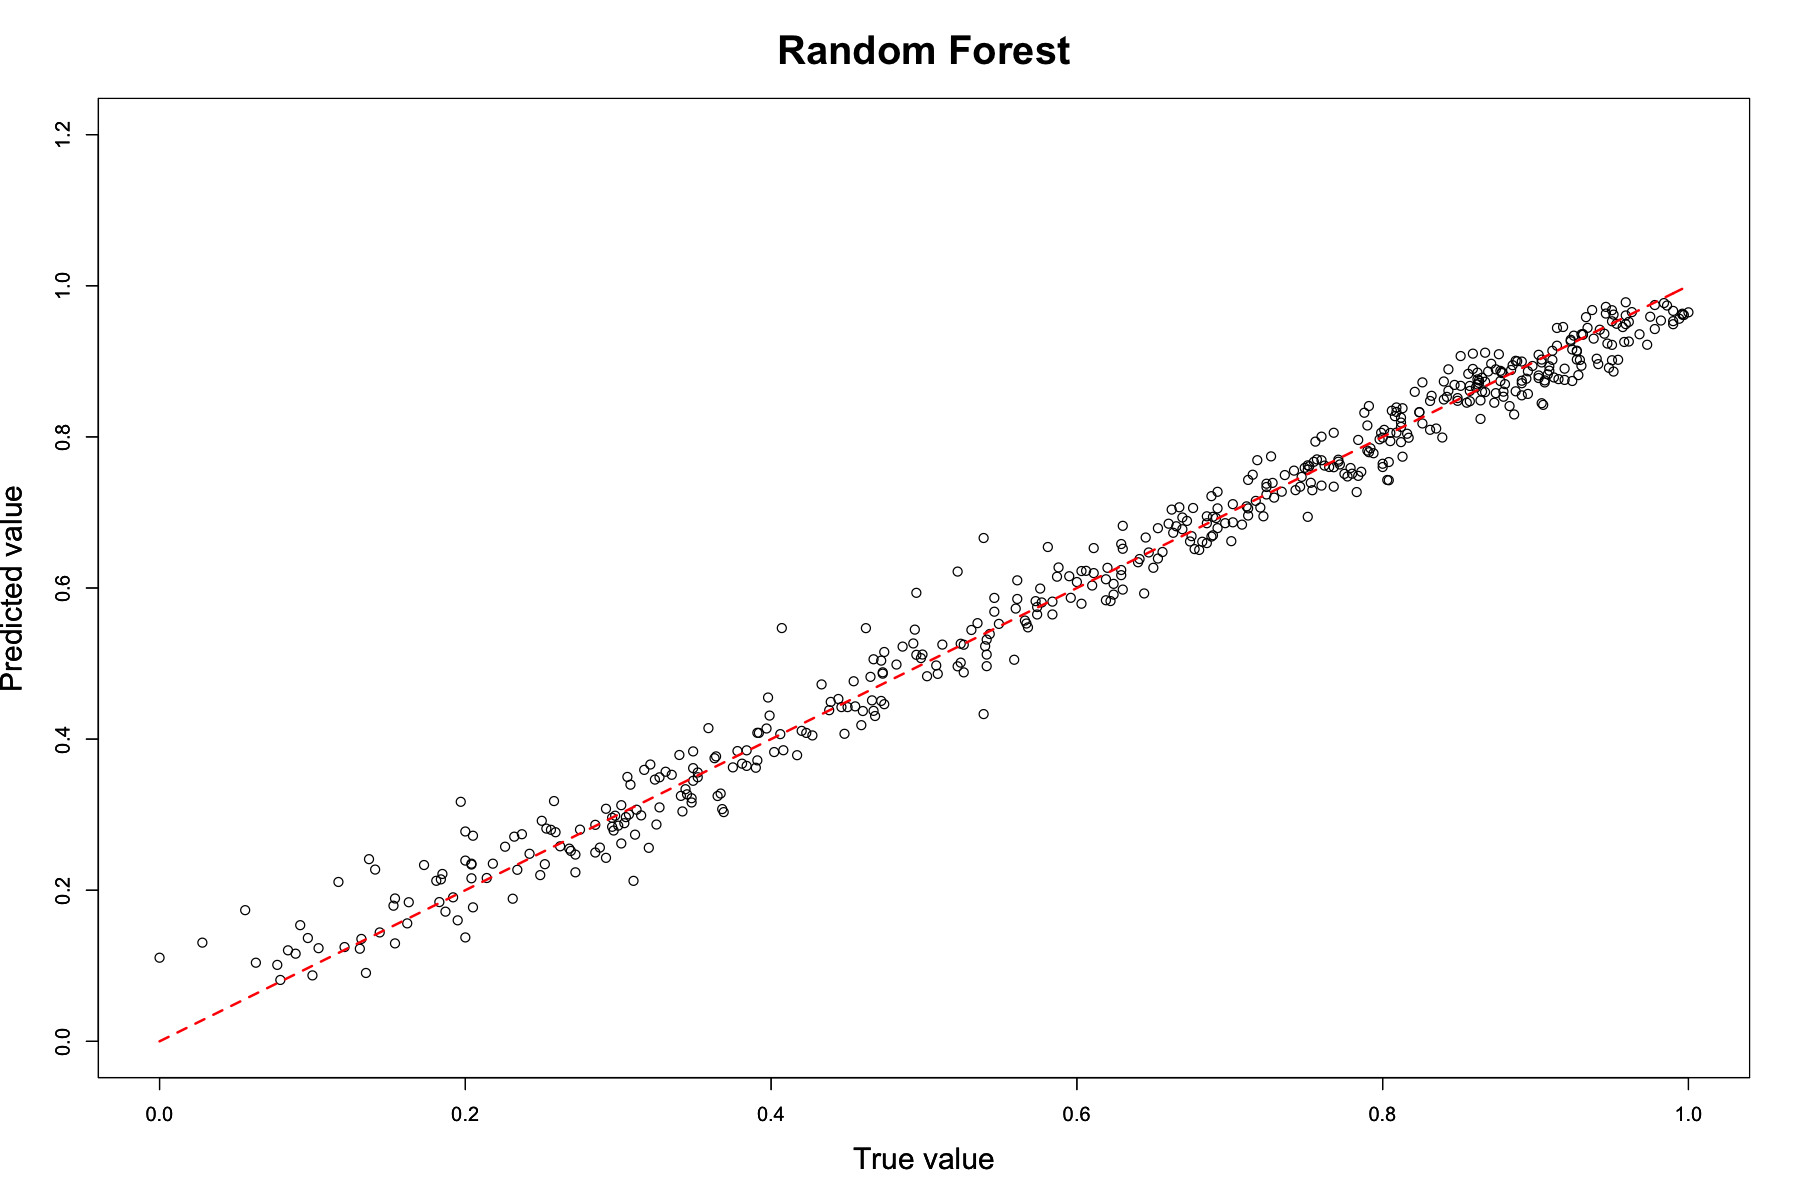
\includegraphics[width = 1.0\textwidth]{Figure/4.2.4-RF.png}
\caption{The predicted Arctic sea ice extent value vs the real Arctic sea ice extent value with Random Forest (200 trees, 5 features). The red referenced dotted line represents the straight line y=x. Mean Square Error (MSE) is 0.00105.}
\label{4.2.4-RF}
\end{figure}



\subsection{Neural Network} %4.2.5

For neural networks, unlike random forests, parameters can be selected based on out-of-pocket errors. Therefore, in the parameter tuning process k-fold is applied to output testing errors for reference. After multiple tests, we finally selected the structure of 5 hidden layers, and 9, 7, 5, 3 and 1 neurons were used in each hidden layer from front to back as following figure shows.

\begin{figure}[htbp]
\centering
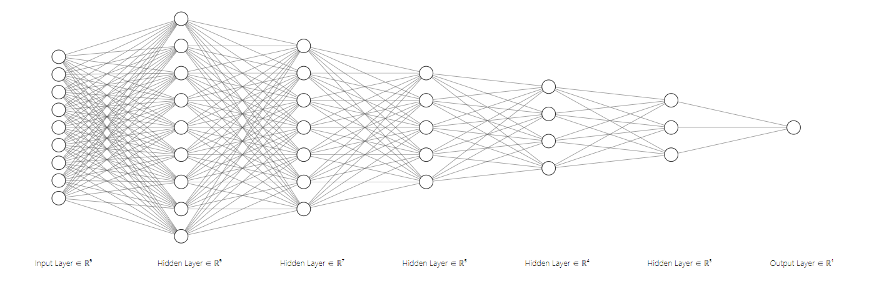
\includegraphics[width = 1.0\textwidth]{Figure/4.2.5-NN-Structure.png}
\caption{Neural Networks Structure}
\label{4.2.5-NN-Structure}
\end{figure}

As for the result, the neural network algorithm achieves excellent performance similar to that of random forest. MSE was slightly lower than the random forest, reaching 1.00104. The fitting diagram (Figure \ref{4.2.5-NN}) also proves that the variance of the neural network model is very low comparing with former algorithms except Random Forest.

\begin{figure}[htbp]
\centering
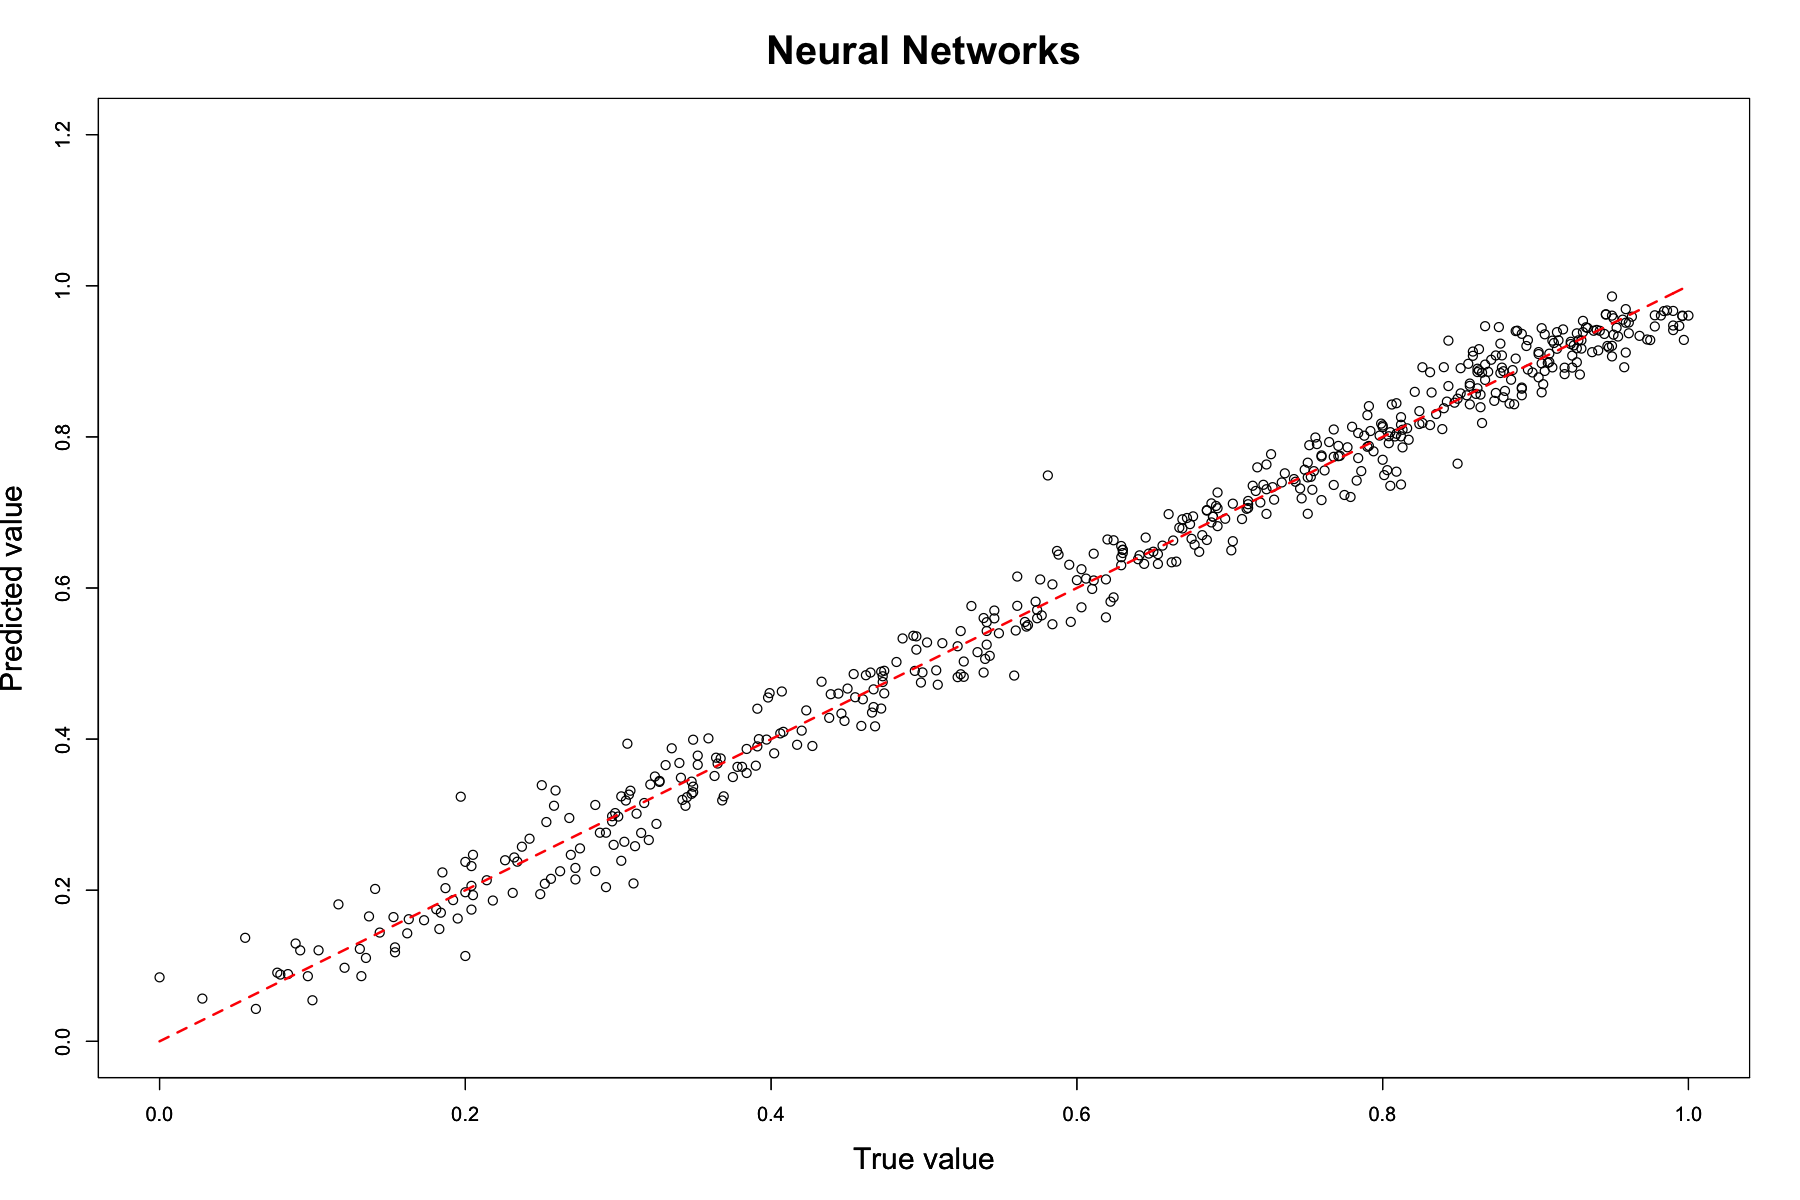
\includegraphics[width = 1.0\textwidth]{Figure/4.2.5-NN.png}
\caption{The predicted Arctic sea ice extent value vs the real Arctic sea ice extent value with Neural Networks (9 neurons, 5 hidden layers with (9,7,5,4,3) nodes respectively). The red referenced dotted line represents the straight line y=x. Mean Square Error (MSE) is 0.00104.}
\label{4.2.5-NN}
\end{figure}



\subsection{Comparison} %4.2.6
Based on the above four models and seven prediction results, all the results are listed and compared here. 

**TABLE**
\begin{figure}[htbp]
\centering
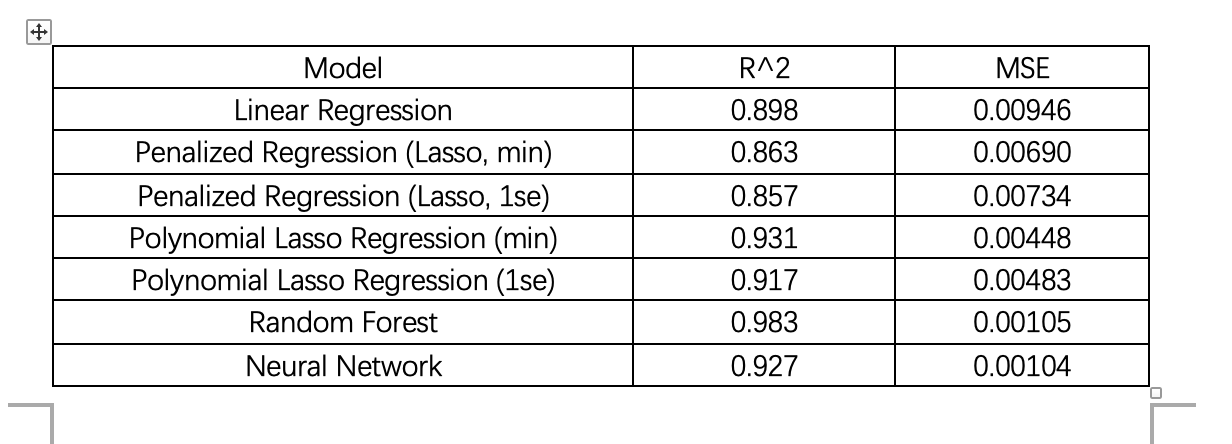
\includegraphics[width = 1.0\textwidth]{Figure/4.2.6-TABLE.png}
\caption{4.2.6-TABLE}
\label{4.2.6-TABLE}
\end{figure}

First, Random Forest, as the best performing model, will be selected for further future predictions. Secondly, it can be found that the model with high $\text{R}^2$ may not perform well, which also proves the existence of over-fitting phenomenon and the necessity of penalise.